% Options for packages loaded elsewhere
\PassOptionsToPackage{unicode}{hyperref}
\PassOptionsToPackage{hyphens}{url}
\documentclass[
]{book}
\usepackage{xcolor}
\usepackage{amsmath,amssymb}
\setcounter{secnumdepth}{5}
\usepackage{iftex}
\ifPDFTeX
  \usepackage[T1]{fontenc}
  \usepackage[utf8]{inputenc}
  \usepackage{textcomp} % provide euro and other symbols
\else % if luatex or xetex
  \usepackage{unicode-math} % this also loads fontspec
  \defaultfontfeatures{Scale=MatchLowercase}
  \defaultfontfeatures[\rmfamily]{Ligatures=TeX,Scale=1}
\fi
\usepackage{lmodern}
\ifPDFTeX\else
  % xetex/luatex font selection
\fi
% Use upquote if available, for straight quotes in verbatim environments
\IfFileExists{upquote.sty}{\usepackage{upquote}}{}
\IfFileExists{microtype.sty}{% use microtype if available
  \usepackage[]{microtype}
  \UseMicrotypeSet[protrusion]{basicmath} % disable protrusion for tt fonts
}{}
\makeatletter
\@ifundefined{KOMAClassName}{% if non-KOMA class
  \IfFileExists{parskip.sty}{%
    \usepackage{parskip}
  }{% else
    \setlength{\parindent}{0pt}
    \setlength{\parskip}{6pt plus 2pt minus 1pt}}
}{% if KOMA class
  \KOMAoptions{parskip=half}}
\makeatother
\usepackage{graphicx}
\makeatletter
\newsavebox\pandoc@box
\newcommand*\pandocbounded[1]{% scales image to fit in text height/width
  \sbox\pandoc@box{#1}%
  \Gscale@div\@tempa{\textheight}{\dimexpr\ht\pandoc@box+\dp\pandoc@box\relax}%
  \Gscale@div\@tempb{\linewidth}{\wd\pandoc@box}%
  \ifdim\@tempb\p@<\@tempa\p@\let\@tempa\@tempb\fi% select the smaller of both
  \ifdim\@tempa\p@<\p@\scalebox{\@tempa}{\usebox\pandoc@box}%
  \else\usebox{\pandoc@box}%
  \fi%
}
% Set default figure placement to htbp
\def\fps@figure{htbp}
\makeatother
\ifLuaTeX
\usepackage[bidi=basic]{babel}
\else
\usepackage[bidi=default]{babel}
\fi
\babelprovide[main,import]{italian}
% get rid of language-specific shorthands (see #6817):
\let\LanguageShortHands\languageshorthands
\def\languageshorthands#1{}
\setlength{\emergencystretch}{3em} % prevent overfull lines
\providecommand{\tightlist}{%
  \setlength{\itemsep}{0pt}\setlength{\parskip}{0pt}}
          \usepackage{cancel}
          \usepackage{comment}
          \usepackage{standalone}
          \usepackage{float}
          \usepackage{multirow}
          \usepackage{subcaption}
          \usepackage{svg}
          \usepackage{tikz}
          \usetikzlibrary{patterns}
          \usepackage[version=4]{mhchem}
          \usepackage{circuitikz}
          \usepackage{pgfplots}
          \usepackage{steinmetz}
          \usepackage{derivative}
          \usepackage{tabularray}
          \usepackage{mathtools}
          \usepackage{siunitx}
          \usepackage[most]{tcolorbox}
          \usepackage{geometry}
          \usepackage{array}
          \usepackage{caption}
          \usepackage{sectsty}
          \usepackage{hhline}
              \geometry{
                  a4paper,
                  total={170mm,257mm},
                  left=20mm,
                  top=20mm,
              }
          \tcbuselibrary{most}
          \newtcolorbox{redbox}[1]{colback=red!5!white, colframe=red!75!black,
          fonttitle=\bfseries, title={#1}}
          \newtcolorbox{greenbox}[1]{colback=green!5!white, colframe=green!75!black,
          fonttitle=\bfseries, title={#1}}
          \newtcolorbox{bluebox}[1]{colback=blue!5!white, colframe=blue!75!black,
          fonttitle=\bfseries, title={#1}}
          \newtcolorbox{orangebox}[1]{colback=orange!5!white, colframe=orange!75!black,
          fonttitle=\bfseries, title={#1}}
\usepackage{bookmark}
\IfFileExists{xurl.sty}{\usepackage{xurl}}{} % add URL line breaks if available
\urlstyle{same}
\hypersetup{
  pdftitle={Appunti Elettronica Digitale},
  pdfauthor={Leonardo Toccafondi},
  pdflang={it},
  pdfsubject={Elettronica},
  hidelinks,
  pdfcreator={LaTeX via pandoc}}

\title{Appunti Elettronica Digitale}
\author{Leonardo Toccafondi}
\date{2024-04-12}

\begin{document}
\frontmatter
\maketitle

{
\setcounter{tocdepth}{2}
\tableofcontents
}
\mainmatter
\chapter{Dispositivi elettronici}\label{dispositivi-elettronici}

\section{Semiconduttori}\label{semiconduttori}

I semiconduttori sono i materiali con cui sono composti i circuiti
integrati. Sono, come suggerisce il nome, materiali in cui il flusso di
corrente \emph{non è libero} (non è un conduttore), ma è
\textbf{presente} (non è un'isolante).\newline In particolare, conducono
in particolari situazioni. Quali sono però i materiali con queste
condizioni?

\begin{itemize}
\tightlist
\item
  \emph{Elementi semiconduttori}: Silicio (\ce{Si}), Germanio (\ce{Ge})
  (Carbonio (\ce{C}), ma composto)
\item
  \emph{Elementi composti}: \ce{GaAs}, \ce{GaN} (Gallio-Arsenico/Azoto)
  In generale sono gli elementi della \(14\textdegree\) colonna della
  tavola periodica o composti a numero medio di elettroni liberi pari a
  4 (dai 3 ai 4).
\end{itemize}

\begin{redbox}{\emph{Silicio}}
Il silicio è il materiale semiconduttore sicuramente più diffuso. \newline
Un atomo presenta 4 elettroni (detti di \emph{valenza}) nello strato più esterno,
ma sua forma cristallina pura del silicio ogni atomo forma un legame covalente\footnote{legame chimico in cui due atomi mettono in comune delle coppie di elettroni.}
con i suoi vicini "più prossimi".
Il cristallo di silicio puro ha inoltre una struttura cristallina matriciale,
che blocca il passaggio di carica. \newline
È da notare che all'aumentare della temperatura, qualche elettrone può rompere il legame
e muoversi liberamente nel cristallo.
\end{redbox}

Per dotare un materiale semiconduttore di conduttività \emph{selettiva}
è necessario \emph{``drogare''} il materiale stesso. Il drogaggio,
quindi, va a \textbf{modificare} la concentrazione di elettroni e di
\emph{lacune} \footnote{Assenza di elettroni dovuta alla
  \textbf{rottura} di un legame. È insieme all'elettrone, un portatore
  di carica nei semiconduttori.}, attraverso questo inserimento di
impurità sostituzionali (ovvero atomi di elementi diversi, i quali si
sostituiscono ad alcuni degli atomi di silicio.) \newline In pratica
andiamo ad aggiungere, in piccole dosi, nel reticolo cristallino
materiali della \(5\textdegree\) colonna (drogaggio di tipo \textbf{n},
hanno 5 elettroni di valenza, sono detti \textbf{donatori}, ad esempio
il fosforo), o elementi della \(3\textdegree\) colonna (tipo \textbf{p},
hanno 3 elettroni di valenza e sono detti \textbf{accettori}, ad esempio
il boro).\newline Tale discrepanza induce la formazione di livelli
energetici aggiuntivi all'interno della banda proibita\footnote{Intervallo
  di energia interdetto agli elettroni, distanza tra la banda di valenza
  di conduzione (nei semiconduttori distanti \(1\si{eV}\)).} o ``gap''
del semiconduttore. Nel primo caso si genera un eccesso di lacune, le
quali si comportano come particelle cariche \emph{positivamente}, mentre
nel secondo si ha un eccesso di elettroni liberi, determinando così una
variazione della conducibilità elettrica intrinseca del materiale.
\newline Non solo, sia le lacune che gli elettroni liberi sono quindi
liberi di muoversi all'interno del semiconduttore!\newline La qualità
del semiconduttore è influenzata dal materiale usato (per esempio Ge è
meglio del \ce{Si}, ma è più raro), che è a sua volta influenzato dal
goal\footnote{(penso voglia dire ``obiettivo perseguito'').}
(elettronica digitale usa \ce{Si}, l'elettronica di potenza il \ce{GaN}
o \ce{SiC}).

Vediamo ora degli elementi in silicio.

\subsection{Giunzione p-n}\label{giunzione-p-n}

Una giunzione pn (o p-n) si forma quando una del materiale
semiconduttore intrinseco\footnote{Puro, quindi privo di un quantitativo
  significativo di drogaggio.} drogato con un drogaggio p (con una
percentuale \(N_{A}\), n.~accettori) viene posta a contatto con altro
materiale semiconduttore drogato con un drogaggio n (con una percentuale
\(N_{D}\), n.~donatori). \newline La concentrazione di ioni dalle
seguenti ``formule'': \[
N_A = \frac{\# acceptors}{vol. unit} \text{ e } N_D=\frac{\# donors}{vol. unit}
\] dove \(N_a\) indica il numero\footnote{Oppure densità di ioni, o
  concentrazione\ldots{}} di ioni di tipo p:`positivo', mentre \(N_d\)
il numero di ioni di tipo n:`negativo'.

Collegando un blocco drogato tipo p ed uno tipo n abbiamo
(idealmente)\footnote{Nella pratica parto da un blocco puro di silicio,
  per poi iniettare a \emph{strati} il drogaggio.}

\begin{figure}[H]
\centering
\begin{tikzpicture}[scale=1.5]
    \draw[very thick](-2,0)--(2,0)--(2,1)--(-2,1)--(-2,0);
    \draw[very thick](0,0)--(0,1);
    \draw[thick](0.5,0)--(0.5,1);
    \draw[thick](-0.5,0)--(-0.5,1);
    \node at (1.25,0.5) {$N$};
    \node at (-1.25,0.5) {$P$};
     % Aggiungiamo le due righe orizzontali
    \draw[thick](-2.5,0.5)--(-2,0.5);
    \draw[thick](2,0.5)--(2.5,0.5);
    \draw[->](-0.25,0.5)--(0.25,0.5)node[above]{$V_0$};
\end{tikzpicture}
\caption{Giunzione pn}
\end{figure}

Il materiale quindi è separato in due zone \emph{nettamente distinte},
senza alterazione della struttura cristallina all'interfaccia delle due
zone. \newline L'abbondanza di lacune in p è, come sappiamo,
corrispondente ad una carenza di elettroni, di cui n \emph{abbonda}. In
altre parole questa diversa \emph{densità} di portatori di carica genera
una \textbf{migrazione} di elettroni da N verso P, detta anche
\emph{diffusione\footnote{Fenomeno che si ritrova in natura qualora vi
  sia uno squilibrio nella distribuzione nello spazio di particelle
  simili.} (elettrica)} \(I_D\) oppure anche \emph{corrente di
diffusione}, che consiste quindi in

\begin{itemize}
\tightlist
\item
  lacune che si diffondono dalla regione (dal semiconduttore) drogata
  con p alla regione n;
\item
  elettroni che si diffondono dalla regione drogata con n alla regione
  p.
\end{itemize}

\begin{quote}
N.B.: Nella zona n i \textbf{portatori maggioritari} di carica sono le
cariche negative, mentre nella zona p sono le cariche positive
\end{quote}

Tale fenomeno carica in modo \emph{positivo} il semiconduttore drogato n
(meno elettroni), e in modo \emph{negativo} il semiconduttore drogato p
(più elettroni). \newline Le lacune che si diffondono dalla regione/zona
p alla n si ricombinano con gli elettroni liberi, \emph{scomparendo}. Di
conseguenza, il numero di elettroni liberi nella zona n
\emph{diminuisce}, quindi non saranno più neutralizzate alcune cariche
fisse positive (atomi donatori). Dal momento che questa ricombinazione
avviene in prossimità della giunzione, accanto a questa si svilupperà
una regione \textbf{svuotata} di elettroni, con cariche fisse positive
non compensate. \newline Analogamente nella zona p otterremo una zona
svuotata dalle lacune e che comprende delle cariche fisse (in questo
caso negative) non compensate.

\begin{figure}[H]
\centering
\begin{subfigure}[t]{0.6\textwidth}
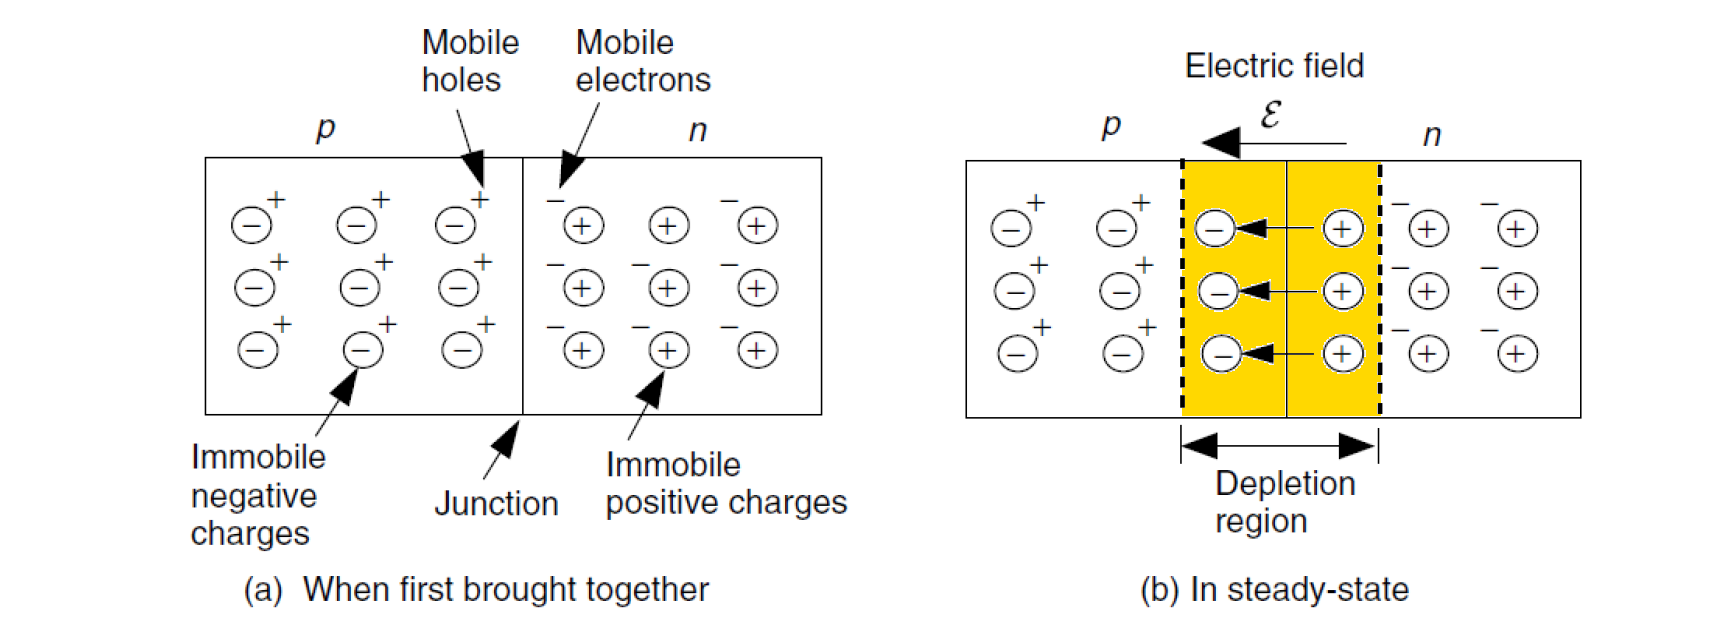
\includegraphics[width=\textwidth,height=\textheight,keepaspectratio]{immagini/1.png}
\caption{Regione di svuotamento}
\end{subfigure}
\begin{subfigure}[t]{0.3\textwidth}
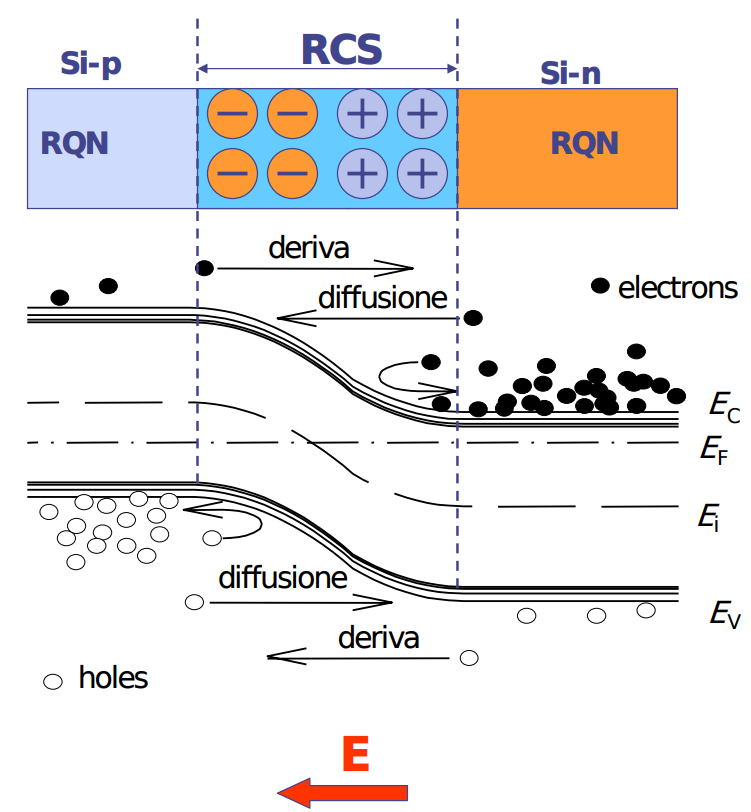
\includegraphics[width=\textwidth,height=\textheight,keepaspectratio]{immagini/pn_equilibrio.png}
\caption{Giunzione pn all'equilibrio}
\end{subfigure}
\end{figure}

Entrambe queste zone danno luogo alla \textbf{regione di
svuotamento}\footnote{Svuotata di portatori \textbf{mobili}} (o di
carica spaziale, in inglese \emph{depletion layer}). Inoltre lo
spostamento delle cariche crea a cavallo della giunzione un campo
elettrico, con la zona n positiva rispetto alla zona p.~La presenza del
campo elettrico comporta la presenza di una differenza di potenziale.
Questa è anche detta \textbf{barriera di potenziale}\footnote{È
  possibile superarla, ma deve essere fornita una differenza di
  potenziale \textbf{esterna}.}, in quanto si oppone ad un'ulterore
diffusione ai portatori di carica soggetti alla spinta della diffusione
(si oppone al movimento di elettroni nella regione p e lacune nella
regione n). Una volta che la corrente di diffusione equivale la corrente
di trascinamento\footnote{Detta anche corrente di deriva (drift), in
  questo caso i portatori si muovono perché \textbf{spinti} dal campo
  elettrico dovuto allo squilibrio di carica.} \(I_S\) raggiungiamo un
\textbf{equilibrio} (dinamico): la presenza del campo elettrico comporta
la presenza di una differenza di potenziale.\newline In genere la
regione di svuotamento non è simmetrica: la seguente equazione regola la
larghezza della regione: \[
x_p N_A = x_N N_D
\] dove \(x_p\) e \(x_n\) sono rispettivamente le \textbf{larghezze}
della regione di svuotamento entro il semiconduttore drogato p e drogato
n.

\begin{figure}[H]
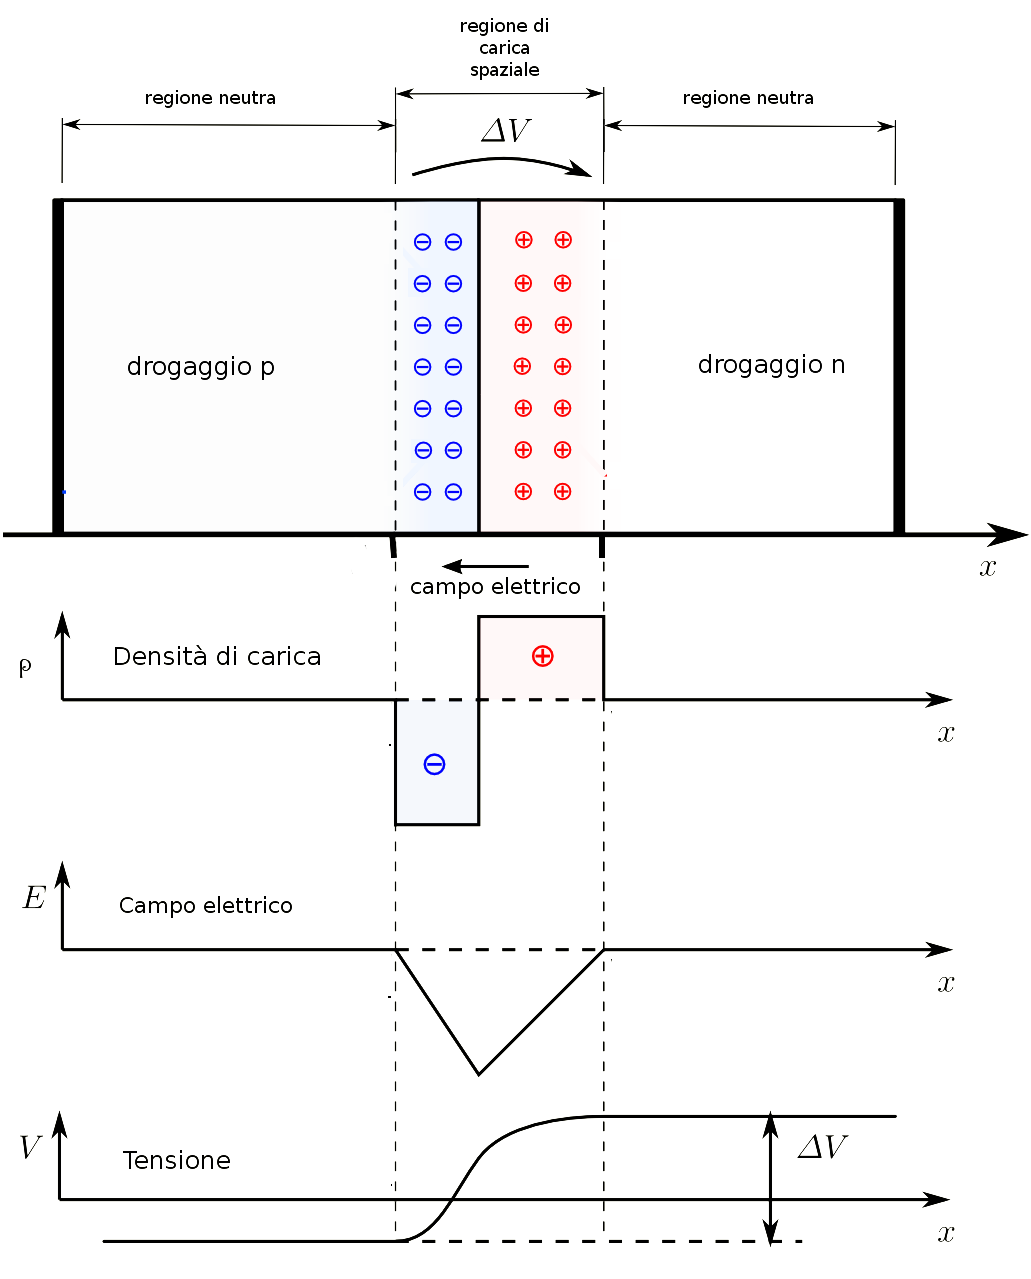
\includegraphics[height=0.5\textwidth, width=!]{immagini/2.png}
\centering
\caption{Grafici relativi al potenziale, al campo elettrico e alla carica nella giunzione pn}
\label{fig:1.3}
\end{figure}

Come si vede nella @fig:1.3 :

\begin{itemize}
\tightlist
\item
  \(N_A > N_D \to\) più è drogata la regione più la regione di
  svuotamento è piccola.
\end{itemize}

\section{I diodi}\label{i-diodi}

Il simbolo circuitale della giunzione p-n, detta
\textbf{diodo}\footnote{Il diodo ideale è un dispositivo che lascia
  passare corrente solo in un senso, con resistenza nulla, e non lascia
  passare corrente nell'altro senso. Il diodo a giunzione approssima
  molto bene un diodo ideale, ed è l'elemento circuitale non lineare più
  importante.} è

\begin{figure}[h]
\begin{centering}
\begin{circuitikz}
  \draw (0,0) node[left]{A} to[diode,color=red] (2,0) node[right]{K};
\end{circuitikz}
\caption{Diodo}
\end{centering}
\end{figure}

dove a sinistra abbiamo un \textbf{anodo} A (dal greco \emph{salita}), e
a destra un \textbf{catodo} K (dal greco \emph{discesa}).\newline Sia la
zone p che la zona n sono munite di un contatto elettrico (detto
\textbf{reoforo}), in modo tale che sia possibile applicarvi una
tensione.

\subsection{Polarizzazione}\label{polarizzazione}

L'applicazione di un potenziale sul diodo viene detta
\textbf{polarizzazione}, e si distingue la:

\begin{itemize}
\tightlist
\item
  Polarizzazione \textbf{diretta} (forward bias): applico un potenziale
  positivo sull'anodo A (lato p) e negativo sul catodo K (lato n). La
  differenza di potenziale applicata ha la polarità \emph{concorde} con
  la barriera di potenziale.

  \begin{itemize}
  \tightlist
  \item
    L'aumento della tensione determina una riduzione della barriera di
    potenziale, e di conseguenza della larghezza della regione di
    svuotamento. In questo modo aumenta il numero di elettroni e di
    lacune capaci di attraversare la giunzione tramite la diffusione.
  \item
    La corrente di diffusione, rispetto a quella di deriva, aumenta
    rapidamente di svariati ordini di grandezza.

    \begin{figure}[h]
    \begin{centering}
    \begin{circuitikz}
    \draw (0,0) node[left]{+} to[diode,color=blue] (2,0) node[right]{-};
    \end{circuitikz}
    \caption{Diodo polarizzato direttamente}
    \end{centering}
    \end{figure}
  \end{itemize}
\item
  Polarizzazione \textbf{indiretta} (reverse bias): applico un
  potenziale negativo sull'anodo e positivo sul catodo. In questo caso
  la polarità della tensione applicata è discorde rispetto a quella
  della barriera di potenziale.

  \begin{itemize}
  \tightlist
  \item
    La regione di svuotamento si allarga, e la tensione di
    polarizzazione richiama le lacune verso il terminale negativo e gli
    elettroni verso il terminale positivo. Quindi l'ampiezza della
    barriera di potenziale aumenta.
  \item
    La corrente di diffusione diminuisce fino ad annullarsi, mentre
    quella di deriva rimane (anche se è molto piccola e varia con la
    temperatura). Quindi quasi nessuna corrente riesce a scorrere.
  \item
    Il campo elettrico incrementa fino ad ottenere il \emph{breakdown}.
  \end{itemize}
\end{itemize}

\begin{figure}[h]
\begin{centering}
\begin{circuitikz}
  \draw[thick] (0,0) node[left]{-} to[diode,color=orange] (2,0) node[right]{+};
\end{circuitikz}
\caption{Diodo polarizzato indirettamente}
\end{centering}
\end{figure}

\subsection{Equazione caratteristica e
breakdown}\label{equazione-caratteristica-e-breakdown}

In generale, la giunzione pn ha un'equazione caratteristica \[
i=I_{S}(e^{\frac{V_d}{nV_t}}-1)
\] detta \textbf{equazione di Shockley}:

\begin{itemize}
\tightlist
\item
  \(V_d\) indica la differenza di potenziale applicati ai capi del
  diodo;
\item
  \(nV_t\) è il potenziale nativo dei diodi (pari a
  \(\SI{0.7}{\volt}\)), o \emph{tensione termica}, pari a
  \(\SI{26}{\mV}\).
\item
  \(I_S\) (o \(I_0\)) è una costante detta \emph{corrente di
  saturazione} (per il \ce{Si} ha valori tra \(10^{-15}\) e
  \(10^{-19} \, \si{\ampere}\))
\end{itemize}

In condizioni di polarizzazione diretta la corrente è trascurabile per
tensioni al di sotto di \(0,5 - 0,6 \si{\volt}\) (per diodi al silicio)
e dopo aver superato la \emph{tensione di soglia} cresce molto
repentinamente\footnote{Per un aumento di corrente di un fattore mille è
  sufficiente un aumento di tensione pari a \(\SI{0.8}{\volt}\). Infatti
  viene assunta \(\SI{0.6}{\volt}\) come tensione di soglia e
  \(\SI{0.8}{\volt}\) come tensione massima.}. \newline Quando il diodo
è in polarizzazione inversa, aumentando la tensione la corrente rimane
costante finché non si raggiunge la cosiddetta \textbf{tensione di
breakdown} (o di rottura). Una volta oltrepassata la corrente aumenta
\colorbox{yellow}{(forse in questo caso \textit{diminuisce})} in maniera
drastica a tensione praticamente costante.

\begin{greenbox}{Il \emph{breakdown}}
Il fenomeno del breakdown è dovuto a:
\begin{enumerate}
\item Effetto \emph{Zener}: prevalente per tensioni di breakdown inferiori alla decina di volt. Quando il diodo è polarizzato
    inversamente e la tensione è compresa tra $0\si{\volt}$ e $V_Z$ (inferiore a zero), si comporta quasi come un circuito aperto,
    seppur continui a scorrere una piccola corrente di saturazione inversa, oltre $V_Z$ la banda di valenza della regione p si
    avvicina talmente tanto alla banda di conduzione che alcuni elettroni si spostano dall'una all'altra;
\item Effetto \emph{valanga} (avalanche): prevalente per tensioni di breakdown superiori alla decina di volt. Si manifesta
    in presenza di campi elettrici \emph{molto elevati}, dovuti alla presenza di una tensione "moderata", ma imposta su distanze
    molto corte.
\end{enumerate}

Solitamente il processo del breakdown è irreversibile, tranne per i diodi Zener, i quali sono ideati per andare in breakdown.
\end{greenbox}
\begin{figure}[H]
    \centering
    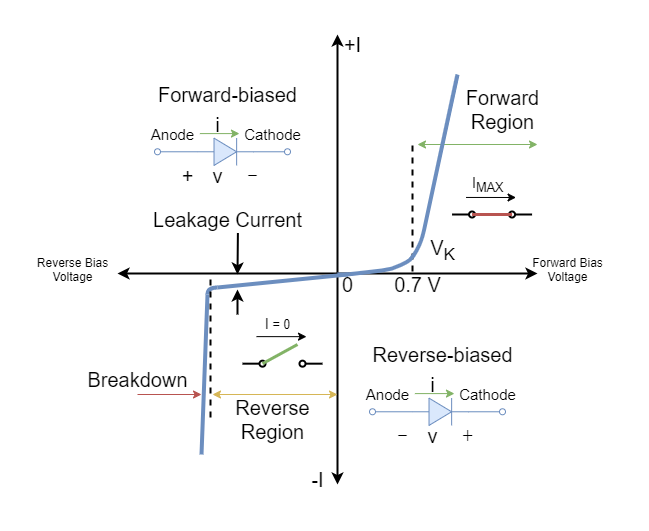
\includegraphics[width=0.5\textwidth]{immagini/iv_pn.png} % replace with your image file
    \caption{Una tipica caratteristica I-V di un diodo a giunzione PN}
    \label{fig:caratteristica_pn}
\end{figure}

\subsection{Diodi Speciali}\label{diodi-speciali}

\subsubsection{Fotodiodi}\label{fotodiodi}

I fotodiodi sono diodi in cui la giunzione è ``scoperta'', o incapsulata
in un materiale trasparente, in quanto vogliamo che sia in grado di
\textbf{emettere} una corrente elettrica sfruttando l'effetto
fotoelettrico. Difatti è un \emph{trasduttore}\footnote{Dispositivo in
  grado di convertire una forma di energia in una diversa.} da un
segnale ottico ad un elettrico. \newline L'equazione caratteristica del
fotodiodo è pari a quella di un diodo normale, con l'aggiunta di un
termine \(I_{ph}\), che rappresenta la corrente
\emph{fotogenerata}\footnote{Risulta proporzionale al flusso di fotoni
  che colpiscono il fotodiodo}: \[
i=I_{S}(e^{\frac{V_d}{nV_t}}-1)-I_{ph}
\]

\begin{center}
\begin{circuitikz}
  \draw (0,0) node[left]{+} to[diode, l_=Diodo normale] (2,0) node[right]{-};
  \draw[pD={}, l_=Fotodiodo] (4,0) node[left]{+} to node[right]{-} (6,0);
\end{circuitikz}
\end{center}

I fotodiodi p-n possono essere utilizzati senza essere polarizzati: sono
adatti per ``applicazioni'' in situazioni di bassa luminosità. Quando
sono illuminati, il campo elettrico nella regione di deplezione aumenta,
producendo la corrente fotogenerata la quale è cresce all'aumentare del
flusso di fotoni. \newline Altrimenti i fotodiodi operano in
\emph{polarizzazione inversa}, in modo tale che i fotoni (del colore
``giusto'') possedano energia sufficiente ad oltrepassare la barriera di
potenziale e a condurre quindi corrente elettrica.

\subsubsection{Led}\label{led}

I \textbf{led} (\emph{light emitting diode}) è un tipo di diodo che
\textbf{converte} energia elettrica in luce. Sono formati da sottili
strati di materiali semiconduttori fortemente drogati, i quali
caratterizzano i diversi colori emessi quando viene applicata una
polarizzazione \emph{diretta}.\newline Da un punto di vista
\emph{costruttivo} i led sono ricoperti da uno strato spesso di
resina\footnote{Epossidica, in inglese \emph{epoxy}.}
\textbf{trasparente} di forma emisferica, sia per proteggere il led
stesso sia per convogliare la luce emessa.

\begin{figure}[h]
\centering
\begin{circuitikz}[american]
\draw[pD={}](0.5,-0.5)to(2.0,-0.5);
\end{circuitikz}
\caption{Simbolo circuitale di un led}
\end{figure}

Applicando quindi una tensione positiva all'anodo, riduciamo la barriera
di potenziale, in modo tale che elettroni e lacune ricombinandosi
generino fotoni pari al gap tra la banda di conduzione e quella di
valenza.

Come si può vedere nella tabella sottostante, al fine di generare un
colore visibile, deve essere fornita una tensione almeno pari a
\(1,5 \si{\volt}\)

\begin{table}[H]
    \centering
    \begin{tabular}{|c|c|c|c|}
    \hline
        \textbf{Semiconduttore composto} & \textbf{$V_{F}$ a $20$ mA} & \textbf{Banda di lunghezza d'onda} & \textbf{Colore} \\ \hline
        GaInN & 4.0V & 450 nm & Bianco \\ \hline
        SiC & 3.6V & 430-505 nm & Blu \\ \hline
        GaAsP & 22V & 585-595 mm & Giallo \\ \hline
        GaAsP & 2.0V & 605-620nm & Ambra \\ \hline
        GaAsP & 1.8V & 630-660nm & Rosso \\ \hline
        GaAs & 1.2V & 850-940nm & Infrarosso \\ \hline
    \end{tabular}
    \caption{Diverse tipologie di led in base al colore prodotto}
\end{table}

\subsubsection{Diodo Schottky}\label{diodo-schottky}

In questa tipologia di diodo la giunzione p-n è data dall'unione del
metallo (che svolge il ruolo della regione p) con un materiale
semiconduttore drogato n.~In questo modo si viene a creare una
\emph{``barriera Schottky''}: questa, a differenza della giunzione p-n
standard, ha una \emph{bassa} tensione di giunzione (o tensione di
soglia). Infatti ai capi di un diodo Schottky si misura solitamente una
differenza di potenziale tra i \(0.15\si{\volt}\) e i
\(0,45 \si{\volt}\): così facendo abbiamo una maggior efficienza e una
maggior velocità di commutazione, riducendo i tempi di
turnoff\footnote{Tempo che passa tra la fine dell'influenza esterna
  (forward bias) ed il momento in cui smette di fluire corrente. È un
  ritardo causato dalla carenza di lacune (\(N_D >> N_A\)), causando un
  accumulo extra di carica in p, la quale sarà rilasciata durante il
  turnoff.}! \newline Inoltre, nella zona della giunzione del metallo,
la zona di svuotamento è \textbf{nulla o quasi inesistente}\footnote{Dal
  lato p.}.

\begin{figure}[h]
\centering
\begin{circuitikz}[american]
\draw[sD={}](0.5,-0.5)to(3.0,-0.5);
\end{circuitikz}
\caption{Simbolo circuitale di un diodo Schottky}
\end{figure}

\subsubsection{Diodo Zener}\label{diodo-zener}

Questa tipologia di diodo lavora in \textbf{breakdown}. Se viene
applicata una polarizzazione \emph{diretta} esso lavora e funziona come
un diodo ``qualsiasi''. Invece, se viene applicata una polarizzazione
\emph{inversa} la tensione di breakdown è ``molto precisa'': in questo
modo se \(V_G < V_Z\) non accade nulla \((V_G = V_Z)\), mentre se
\(V_G \geq V_Z\) allora il diodo va in breakdown e su esso scorre una
corrente. Ho quindi una tensione di uscita \emph{stabilizzata}
\((V_O = V_Z)\).\newline Nel circuito della figura seguente la
resistenza è molto importante, in quanto se non fosse presnete
\(i_R = \frac{V_G - V_i}{R}\), ma \(R\to0\) e quindi \(i_{R}\to \infty\)

\begin{figure}[H]
\centering
\resizebox{0.25\textwidth}{!}{%
\begin{circuitikz}
\tikzstyle{every node}=[font=\normalsize]
\draw (0,2.25) to[american voltage source, invert] (0,0.25);
\draw (0,2.25) to[R] (3,2.25);
\draw[zzD={}](3,0.25) to(3,2.25);
\draw (0,0.25) to[short] (3,0.25);
\draw (2.75,2.25) to[short, -o] (4,2.25);
\draw (3,0.25) to (3,0) node[ground]{};
\draw [->, >=Stealth] (1,1.75) -- (2,1.75);
\node [font=\normalsize] at (1.5,1.5) {$i_{R}$};
\node [font=\normalsize] at (0.75,0.75) {$V_{G}$};
\node [font=\normalsize] at (4.5,2.25) {$V_{o}$};
\end{circuitikz}
}%

\label{fig:my_label}
\caption{Schema di un diodo Zener}
\end{figure}

\chapter{I transistor}\label{i-transistor}

\section{Introduzione}\label{introduzione}

Un transistor è un dispositivo a semiconduttori utilizzato per
interrompere (commutare) o amplificare segnali elettrici, come se fosse
una \textbf{valvola}\footnote{Infatti sono andate a sostituire le
  \emph{valvole termoioniche}, o \emph{tubo a vuoto}.}: in pratica
regola la corrente che scorre in una maglia (quella in uscita al
circuito) tramite la tensione applicata ad un'altra (ovvero quella in
ingresso al circuito). \newline Quando viene utilizzato come
interruttore, un transistor è un dispositivo logico a \emph{due stati}:
ON e OFF (binario 1 e 0). Sulla base di questo vengono realizzate
\emph{porte logiche} più complesse, quali AND, OR, NOT, le quali a loro
volta sono impiegate per realizzare tutti quei dispositivi che
compongono la parte \textbf{digitale} dell'elettronica (famiglie
logiche, memorie etc.). \newline Invece, quando viene utilizzato come
modulatore di corrente, un transistor è a ``semplicemente'' un
\textbf{amplificatore}\footnote{Può essere sia un amplificatore di
  potenza che di tensione.}.

\section{Bipolar Junction Transistor: i
BJT}\label{bipolar-junction-transistor-i-bjt}

A differenza dei diodi a giunzione, i \emph{transistor bipolari}
utilizzano tre strati di materiali semiconduttori, in pratica otteniamo
due diodi posti in \emph{antiserie}\footnote{Antiserie indica, per
  bipoli \textbf{polarizzati}, una connessione in serie (quindi un solo
  punto di contatto), in cui le polarità dei terminali vengono
  accoppiate per segni uguali}, in modo tale da ``condividere'' uno
strato.\footnote{Oppure possiamo anche dire che sono due giunzioni p-n
  poste l'una di seguito all'altra e orientata in senso inverso, andando
  poi a costituire tre regioni \emph{consecutive}.} \newline Ad ogni
strato sarà associato un \emph{terminale\footnote{Si può esprimere anche
  come \emph{elettrodo}}}: quello che sarà detto \textbf{base}, che a
sua volta separa due terminali drogati con gli stessi materiali (opposti
al materiale della base), che saranno detti rispettivamente
\textbf{collettore} ed \textbf{emettitore}. \newline I dispositivi BJT
sono dispositivi \emph{bipolari} in quanto il processo di conduzione
coinvolge portatori di \emph{entrambe le polarità}. \newline La
struttura di un transistor BJT può essere realizzata in due modi: quello
\textbf{npn} e quello \textbf{pnp}. È importante notare come in un
transistor la zona dell'emettitore è significativamente più drogata di
quelle di base e di collettore; si indica infatti con p+ nei transistori
pnp e con n+ nei transistori npn.

\begin{figure}[H]
\centering
    \begin{subfigure}[b]{0.45\textwidth}
    \centering
    \begin{circuitikz}
        \draw (0,0) node[npn](Q){};
        \draw[thick] (-0.25,0) circle(0.5);
        \draw (-1.5,0)node[left]{$B$}to[short,i=$I_B$,*-](Q.B);
        \draw (0,1.5)node[above]{$C$}to[short,i_=$I_C$,*-](Q.C);
        \draw (Q.E)to[short,i_=$I_E$,-*](0,-1.5)node[below]{$E$};
        
        \draw[->](0.25,-1.375)to[out=45,in=315](0.25,1.375);
        \draw[->](-0.25,-1.5)to[out=180,in=270](-1.5,-0.25);
        \draw[->](-0.25,1.5)to[out=180,in=90](-1.5,0.25);
        \node at (1.3,0){$V_{CE}$};
        \node at (-1.375,-1.375){$V_{BE}$};
        \node at (-1.375,1.375){$V_{CB}$};

    \end{circuitikz}
    \caption{Transistor npn}
    \end{subfigure}
    \begin{subfigure}[b]{0.45\textwidth}
    \centering
    \begin{circuitikz}
        \draw (0,0) node[pnp](Q){};
        \draw[thick] (-0.25,0) circle(0.5);
        \draw (-1.5,0)node[left]{$B$}to[short,i<=$I_B$,*-](Q.B);
        \draw (0,-1.5)node[below]{$C$}to[short,i<=$I_C$,*-](Q.C);
        \draw (Q.E)to[short,i<=$I_E$,-*](0,1.5)node[above]{$E$};
        
        \draw[->](0.25,-1.375)to[out=45,in=315](0.25,1.375);    
        \draw[<-](-0.25,1.5)to[out=180,in=90](-1.5,0.25);
        \draw[<-](-0.25,-1.5)to[out=180,in=270](-1.5,-0.25); %VBC
        \node at (1.3,0){$V_{EC}$};
        \node at (-1.375,1.375){$V_{EB}$};
        \node at (-1.375,-1.375){$V_{CB}$};
    \end{circuitikz}
    \caption{Transistor pnp}
    \end{subfigure}
    \caption{Transistor BJT}
\end{figure}

\begin{figure}[H]
    \centering
    \begin{subfigure}[b]{0.45\textwidth}
        \centering
        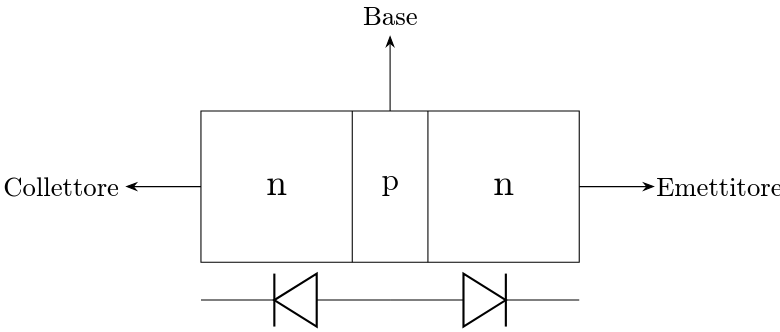
\includegraphics[width=\textwidth]{immagini/npn.png}
        \caption{Caption for image 1}
        \label{fig:image1}
    \end{subfigure}
    \hfill
    \begin{subfigure}[b]{0.45\textwidth}
        \centering
        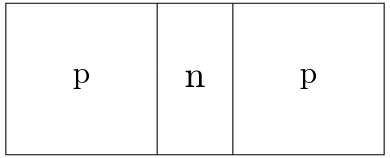
\includegraphics[width=0.75\textwidth]{immagini/pnp.png}
        \caption{Caption for image 2}
        \label{fig:image2}
    \end{subfigure}
    \caption{Overall caption for the figure}
    \label{fig:subfigures}
\end{figure}

Come è possibile notare dalle figure precedenti, da un punto di vista
circuitale i transistor BJT sono rappresentati utilizzando 3 terminali:
\(\to\) nel simbolo indica la giunzione (e ne è riportata solo una),
mentre le frecce indicano i versi delle tensioni (dove sono maggiori).
Parlando del transistor npn, per quanto riguarda le correnti abbiamo che
all'equilibrio \(I_B + I_C = I_E\), ed \(I_B, I_C\) sono entranti,
mentre \(I_E\) è uscente.

Per entrambe le tipologie di BJT, da un punto di vista costruttivo
valgono queste regole:

\begin{enumerate}
\def\labelenumi{\arabic{enumi}.}
\tightlist
\item
  La regione dell'emettitore è altamente drogata e ha il compito di
  emettere o iniettare portatori di corrente nella regione di base. Nei
  transistor npn, l'emettitore di tipo n immette elettroni liberi nella
  base, mentre nei transistor pnp, l'emettitore di tipo p introduce
  lacune nella base.
\item
  La base è sottile e leggermente drogata. La maggior parte dei
  portatori di corrente iniettati nella regione di base si muove verso
  il collettore senza fuoriuscire dal conduttore della base.
\item
  La regione del collettore è moderatamente drogata ed è la più grande
  all'interno del transistor. La sua funzione consiste nel raccogliere o
  attrarre i portatori di corrente iniettati nella regione di base.
\end{enumerate}

\section{Bipolar Junction Transistor: i
BJT}\label{bipolar-junction-transistor-i-bjt-1}

Il transistor BJT è stato il primo transistor ad essere prodotto su
larga scala, precedendo di una decade l'introduzione dei transistor ad
\textbf{effetto di campo}.

I BJT sono un dispositivo a semiconduttore a \textbf{tre} terminali,
realizzato tramite due giunzioni p-n.~Sono \textbf{bipolari} in quanto
il processo di conduzione coinvolge portatori di \emph{entrambe le
polarità}: quindi sia lacune che elettroni. \newline La realizzazione
fisica consiste nell'utilizzo di tre strati di materiale semiconduttore,
collegati ognuno ad un proprio terminale: abbiamo due strati esterni
composti con lo stesso materiale drogante (\textbf{collettore} ed
\textbf{emettitore}), ed un secondo strato posto tra gli altri due
all'interno del quale viene introdotto un materiale drogante opposto
(\textbf{base}). Così facendo otteniamo due giunzioni p-n: una
base-emettitore ed una base-collettore.

\begin{redbox}{\emph{Configurazione a diodi}}
In generale un transistor BJT è \textbf{quasi equivalente }a porre due diodi in antiserie\footnote{Antiserie indica, per bipoli polarizzati, una connessione in serie (quindi un solo punto di contatto), in cui le polarità dei terminali vengono accoppiate per segni uguali}. In realtà è più vicina una configurazione di due giunzioni p-n poste l'una di seguito all'altra e orientate in senso inverso (ognuna delle quali con la propria regione di svuotamento). Questo perché per \emph{far funzionare} il transistor BJT è necessaria la presenza di un'\emph{unica} regione di base, che svolge un ruolo cruciale nel controllo della corrente. Quando si affiancano due diodi, l'interazione tra le loro giunzioni non riproduce le caratteristiche di amplificazione e controllo della corrente tipiche di un BJT, in quanto l'introduzione di un metallo nel circuito non permette la corretta gestione delle correnti e delle tensioni necessarie per il funzionamento del transistor: non vi è il campo elettrico necessario a far passare gli elettroni da un diodo all'altro passando per il filo metallico.
\end{redbox}

È possibile realizzare la struttura in due diverse modalità:

\begin{itemize}
\tightlist
\item
  tipo \textbf{npn}
\item
  tipo \textbf{pnp}
\end{itemize}

I transistor npn sono usati più frequentemente. Inoltre le regole ed i
risultati ottenuti possono essere estesi ai transistor pnp modificando
opportunamente i versi di tensioni e correnti.

\subsection{Il BJT npn}\label{il-bjt-npn}

Un BJT npn è formato da due sezioni di tipo n (emettitore e collettore),
e da una di tipo p.~ Di fondamentale importanza per la fabbricazione di
un BJT è lo \emph{spessore della base}. Infatti deve essere il più
\textbf{sottile} possibile, senza ottenere un corto circuito tra le
regioni del collettore e dell emettitore.

In base alle polarizzazioni applicate alle giunzioni base-collettore e
base-emettitore, otteniamo 4 \textbf{regioni di funzionamento} del
transistor BJT:

\begin{table}[h]
\centering
\begin{tabular}{|c|c|c|}
\hline
\multicolumn{2}{|c|}{\textbf{Polarizzazione delle giunzioni}} & \multirow{2}{*}{\textbf{Regione di funzionamento}} \\ \cline{1-2}
\emph{B-E} & \emph{B-C} &  \\ \hline
Inversa & Inversa & Cutoff (Spento) \\ \hline
Diretta & Inversa & Attiva Diretta \\ \hline
Diretta & Diretta & Saturazione \\ \hline
Inversa & Diretta & Attiva Inversa \\ \hline
\end{tabular}
\caption{Regioni di funzionamento in base alla polarizzazione delle giunzioni}
\label{tab:reg-bjt}
\end{table}

\subsubsection{Regioni di funzionamento}\label{regioni-di-funzionamento}

\paragraph{Cutoff}\label{cutoff}

In questa regione il transistor è \emph{spento}. Entrambe le giunzioni
sono polarizzate inversamente: le rispettive tensioni sono ambedue
\textbf{sotto soglia}. In particolare \(V_{BE}<V_{\text{soglia}}\) e
\(V_{BC}<0\). \newline Dato che la giunzione BE non è polarizzata
\(\to i_B = 0\). Inoltre, dato che tutte le giunzioni sono polarizzate
inversamente, anche la corrente del collettore è \emph{nulla}.
\(\to i_C = 0\) \newline Nel grafico, la corrente non è esattamente
nulla dato che secondo la legge di \(I_D\) in una giunzione con
polarizzazione inversa la corrente vale \(I_O\).

\begin{quote}
In definitiva non vi è conduzione.
\end{quote}

\paragraph{Attiva diretta}\label{attiva-diretta}

In questa regione la giunzione BE è polarizzata \emph{direttamente},
mentre la giunzione BC è polarizzata inversamente. Significa che:

\begin{itemize}
\tightlist
\item
  \(V_{BE} > V_{\text{soglia}}\)
\item
  \(V_{BC} < 0\)
\end{itemize}

La corrente \(I_B >0\), e nonostante la tensione della giunzione BC sia
negativa, \(I_C= h_{fe}I_{b}\). \newline Dunque gli elettroni dovrebbero
ricombinarsi e ``richiudersi'' verso la base. Tuttavia, sapendo che la
base è ``corta'' gli elettroni raggiungono il collettore prima di
ricombinarsi, il quale li prende (forse meglio dire li accetta), in
quanto possiede un potenziale \emph{positivo}. È da notare che comunque
non tutti gli elettroni riescono ad attraversare tutto il transistor,
statisticamente alcuni si ricombinano con le lacune presenti nella
regione della base.

Il \footnote{È una funzione di.}\textbf{guadagno\footnote{In inglese è
  \textbf{gain}.} del transistor di corrente} è
\(h_{fe}=\frac{I_C}{I_B}\). Il transistor ha una funzione di
\emph{amplificatore} della corrente di base nel caso in cui \(h_{fe}\)
sia un valore alto: ciò lo rende \textbf{\emph{``attivo''}}

\begin{quote}
In questa regione funge da generatore di corrente controllato in
corrente.
\end{quote}

\paragraph{Saturazione}\label{saturazione}

In questa regione anche la giunzione BE è polarizzata direttamente:

\begin{itemize}
\tightlist
\item
  \(V_{BE}< V_{\text{soglia}}\)
\item
  \(V_{CE}<V_{CE -sat}\)
\end{itemize}

Se vale quest'ultima condizione (la tensione della giunzione BE è bassa)
allora anche BC è polarizzata direttamente. Per lo stesso motivo gli
elettroni non vengono ``raccolti'' dal collettore, tendendo a rimanere
nella base:

\begin{itemize}
\tightlist
\item
  \(I_{B}>0\)
\item
  \(I_C < h_{fe}\ I_{B}\)
\end{itemize}

\begin{quote}
È da notare come in questa configurazione/regione otteniamo una tensione
in uscita \textbf{costante} \(V_{CE - sat}\)
\end{quote}

\paragraph{Regione attiva inversa}\label{regione-attiva-inversa}

In questo caso \(V_{BE}<0\) e \(V_{BC} > V_{\text{soglia}}\). Quindi gli
elettroni si spostano nel collettore. In questo caso il *guadagno di
corrente è \(\leq 1\): \(\ I_{e} \simeq - I_{B}\).

\begin{quote}
Otteniamo un guadagno di corrente molto basso (tipicamente \(\leq 1\))
\end{quote}

\begin{figure}
\centering
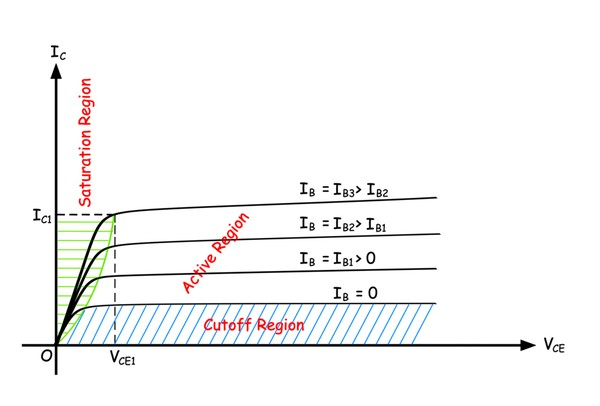
\includegraphics[width=0.7\linewidth,height=\textheight,keepaspectratio]{assets/imgs/curva_bjt_npn.png}
\caption{Curva BJT.}
\end{figure}

In questo grafico sono rappresentate delle curve che riportano gli
andamenti di \(I_C\) in funzione di \(V_{CE}\) con \(I_B\).

\subsection{Layout planare di un transistor
NPN}\label{layout-planare-di-un-transistor-npn}

\begin{figure}[H]
\centering
\resizebox{0.25\textwidth}{!}{%
\begin{circuitikz}
\tikzstyle{every node}=[font=\large]
\draw [thick, fill=blue!20](0,4.25) rectangle (5,0.25);
\draw [thick, fill=red!20]  (1,4.25) rectangle (4,2.25);
\draw [thick, fill=blue!20] (2,4.25) rectangle (3,3.25);
\draw [short] (0,1.25) -- (5,1.25);
\draw [short] (2.5,0.25) -- (2.5,-0.25);
\draw [short] (2.5,4.75) -- (2.5,4.25);
\draw [short] (3.5,4.75) -- (3.5,4.25);
\node [font=\large] at (2.5,0.75) {n+};
\node [font=\large] at (2.5,1.75) {n};
\node [font=\large] at (2.5,2.75) {p};
\node [font=\large] at (2.5,3.75) {n+};
\node [font=\normalsize] at (2.5,5) {Emettitore};
\node [font=\normalsize] at (3.75,5) {Base};
\node [font=\large] at (2.5,-0.5) {Collettore};
\end{circuitikz}
}%
\centering
\caption{Configurazione planare di un BJT npn}
\label{fig:my_label}
\end{figure}

Come mostra anche lo schema, da un punto di vista fisico il layout
planare di un transistor BJT npn \emph{non è simmetrico}: questo sia per
il drogaggio, sia per la realizzazione del dispositivo stesso.
L'emettitore è molto piccolo e molto drogato, mentre le regioni della
base e del collettore sono (viceversa) molto grandi e poco drogate.
\newline I contatti della base, dell'emettitore e del collettore sono
\emph{metallici} (se legati a zona n viene un diodo di silicio). Dato
che i materiali \(n^{+}\) sono molto drogati la regione di svuotamento è
molto piccola e gli elettroni la possono attraversare come se non ci
fosse.

\subsection{Il BJT pnp}\label{il-bjt-pnp}

È un dispositivo \emph{complementare} al pnp: valfolo le stesse
equazioni, ma tensioni e correnti sono \textbf{opposte} \newline Sia le
prestazioni che il guadagno sono \textbf{minori}, perché i portatori in
movimento sono le \emph{lacune}, più lente rispetto agli elettroni.

\subsection{Transistor ``speciali''}\label{transistor-speciali}

\subsubsection{Foto transistor}\label{foto-transistor}

Il phototransistor è caratterizzato da una corrente di base
\emph{``photo-generated''}\footnote{In questo caso la corrente di base è
  sostituita dall'intensità luminosa.}. Il resto dei parametri di lavoro
sono gli stessi un un normale BJT. \[
I_C = k \cdot P_{L}
\] dove \(P_L\) è la potenza luminosa.\newline È importante che il
dispositivo si trovi in regione attiva: per questo sarà inserito un
resistore dal lato del collettore per evitare di andare in saturazione.

\begin{figure}[H]
\centering
\begin{circuitikz}[american]
\draw(1.0,-1.0) node[npn,photo,scale=0.59](Q1){};
\draw[short](Q1.C)to(1.0,-0.5);
\draw[short](Q1.E)to(1.0,-1.5);
\draw(2.0,-1.0) node[pnp,photo,scale=0.59](Q2){};
\draw[short](Q2.E)to(2.0,-0.5);
\draw[short](Q2.C)to(2.0,-1.5);
\end{circuitikz}
\caption{Un fototransistor npn ed uno pnp}
\end{figure}

\begin{figure}[H]
\centering
\resizebox{0.25\textwidth}{!}{%
\begin{circuitikz}
\tikzstyle{every node}=[font=\normalsize]
\draw (0,2) to[R] (0,0);
%\draw (0,0) to[npn, photo] (0,-2);
\draw(0.0, 0.0) node[npn,photo,scale=0.7](0,-3){};
%\draw[short={}](0.0,-2)to(-2.0,-3.0);
\node at (0,2) [circ] {};
\node [font=\normalsize] at (0.5,2) {$V_{CC}$};
\node [font=\normalsize] at (0.5,1) {$R$};
\node [font=\normalsize] at (2.25,0) {$V_{CE} = V_{CC} - R \cdot I > 0.2$};
\end{circuitikz}
}%

\label{fig:my_label}
\caption{Schema con fototransistor npn}
\end{figure}

\section{I transistor MOS}\label{i-transistor-mos}

I \textbf{MOSFET} (\emph{Metal Oxide Semiconductor Field Effect
Transistor}) sono una tipologia di transistor appartenente ai transistor
ad \textbf{effetto di campo}: non si basano sulle proprietà delle
giunzioni p-n.

\begin{greenbox}{\emph{I transistor ad effetto di campo}}
I transistor ad effetto di campo sono caratterizzati dalla possibilità di controllare la \textbf{conduttività elettrica del dispositivo}, ovvero la quantità di corrente elettrica che attraversa il dispositivo stesso, attraverso la formazione di un \emph{campo elettrico}
all'interno di esso. \newline
Possono essere realizzati in diverse modalità: 
\begin{enumerate}
\item JFET: ovvero Junction-Fet, realizzato con una giunzione p-n come elettrodo "rettificante";
\item MESFET: abbreviazione di Metal Semiconductor FET realizzato tramite una giunzione Schottky raddrizzante metallo-semiconduttore; 
\item MOSFET: il più comune.
\end{enumerate}
\end{greenbox}

I MOS sono strutturati con più \emph{strati di materiali sovrapposti}:
metallo, ossido di silicio \((\ce{SiO_2})\) e del silicio, o di tipo
\(p\) o di tipo \(n\). Si utilizza l'ossido come un \emph{isolante}, non
permettendo quindi il passaggio di cariche elettriche tra il metallo ed
il semiconduttore.\newline Uno dei pregi dei transistor di tipo
\emph{MOS} è il \textbf{consumo}: un BJT ha un consumo di energia
\emph{costante} nel tempo (dal momento che deve mantenere la
polarizzazione), mentre un transistor MOS consuma solo durante le
\emph{transizioni}.

Come per i transistor a giunzione, a seconda del drogaggio possiamo
ottenere due tipologie diverse di transistor MOS: i nmos e i pmos.
\newline In particolare, sono dispositivi \emph{controllati in
tensione}.

\subsection{N-MOS}\label{n-mos}

Nell'N-MOS (a canale \(P\)), il silicio è di tipo \(n\): il drogaggio
\(n+\) favorisce il contatto ohmico\footnote{Un \emph{contatto ohmico} è
  una giunzione elettrica tra un metallo e un semiconduttore che non ha
  proprietà rettificanti (non trasforma un segnale alternato in uno
  continuo). La caratteristica principale è avere una curva
  corrente-tensione \(I-V\) lineare, come prevista dalla legge di Ohm.}
con l'alluminio. Le definizioni delle correnti e delle tensioni
equivalgono quelle dei transistor NPN.

\begin{figure}[H]
\centering
\resizebox{0.7\textwidth}{!}{%
\begin{circuitikz}
\tikzstyle{every node}=[font=\LARGE]

\draw[thick, fill=red!20]   (0,7.25) rectangle (11,3.25); %rettangolo principale
\draw[thick, fill=yellow!20]   (4,8.25) rectangle (7,7.25); %ossido
\draw[thick, fill=blue!20]   (2,7.25) rectangle (4,6.25); %n+
\draw[thick, fill=red!60]   (4,9.25) rectangle (7,8.25); %metal gate
\draw[thick, fill=blue!20]   (7,7.25) rectangle  node {\LARGE n+} (9,6.25);%n+
\node [font=\Large] at (5.5,5.25) {P};
\node [font=\Large] at (3,6.75) {n+};
\node [font=\Large] at (5.5,8.75) {Metal gate};
\node [font=\Large] at (5.5,7.75) {Ossido di S};
\node [font=\Large] at (3,8.5) {Source};
\draw [short] (3,8.25) -- (3,7.25);
\draw [short] (8,8.25) -- (8,7.25);
\node [font=\Large] at (8,8.5) {Drain};
\draw [short] (5.5,10.25) -- (5.5,9.25);
\node [font=\Large] at (5.5,10.5) {Gate};
\draw (20,8.5) to[Tnmos, transistors/scale=1.02] (20,4.5);
\draw  (20.25,6.5) circle (1cm);
\draw [<->, >=Stealth] (12,5.75) -- (16,5.75);
\draw [->, >=Stealth] (21.75,5.25) .. controls (22.5,6.5) and (22.25,7.25) .. (21.75,7.75)  node[midway, right] {$V_{CE}$};
\draw [->, >=Stealth] (20,8.5) -- (20,7.5);
\draw [->, >=Stealth] (21,6.5) -- (20.5,6.5);
\draw [->, >=Stealth] (18.5,6.25) -- (19.25,6.25);
\draw [short] (19.25,6.25) -- (19.75,6.25);
\draw [short] (19.75,6.75) -- (19.75,6.25);
\draw [->, >=Stealth] (20,5.5) -- (20,4.75);
\draw [short] (20,4.5) -- (21,4.5);
\node [font=\Large] at (17.75,6.25) {Gate};
\node [font=\Large] at (20,8.75) {Drain $\sim$ D};
\node [font=\Large] at (22.25,4.5) {Source $\sim$ S};
\node [font=\Large] at (20.5,7.75) {$I_D$};
\node [font=\Large] at (20,4) {$I_S$};
\draw [->, >=Stealth] (19.5,4.75) .. controls (18.75,5) and (18.75,5.25) .. (18.25,6)node[midway, right] {$V_{GS}$};
\draw [->, >=Stealth] (17.75,6) -- (17.75,5);
\node [font=\Large] at (17,4.5) {Terminale di controllo};

\node[font=\large, text=blue] at (5.5, 6.75) {- - Canale - -}; 
\end{circuitikz}
}%

\label{fig:my_label}
\caption{Sezione di un transistor N-MOS.}
\end{figure}

È da notare come solitamente il metallo utilizzato sia l'alluminio,
anche se a volte può essere del silicio molto drogato. L'ossido, invece,
è ossido di silicio.\newline In generale qualsiasi MOSFET (quindi anche
un N-MOS) ha tre terminali: \textbf{\emph{source}} (emettitore),
\textbf{\emph{gate}} (base) e \textbf{\emph{drain}}
(collettore)\footnote{Di solito la regione di silicio drogato più grande
  (ad esempio la regione p nel N-MOS), viene detta \emph{bulk}.}.

All'atto pratico si ha la corrente del gate sempre \textbf{nulla} (in
regime continuo; essenzialmente solo col potenziale ``fermo'':
\(i_{G}=\frac{dV}{dt}\cdot C\)). L'ossido ha la funzione di isolante,
inoltre la lastra (di metallo) è sottile \((\approx 10 nm)\), la quale
\emph{blocca}\footnote{Infatti anche per quanto riguarda lo schema del
  circuito il gate è isolato rispetto agli altri due terminali.} il
passaggio di corrente dal gate al blocco sottostante, formando una
struttura di un \emph{condensatore a facce piane}.\newline Come detto in
precedenza la struttura di un transistor N-MOS è simile ad un
condensatore, dove le piastre sono il gate, mentre la piastra sotto è
l'ossido. Applicando quindi una tensione positiva in GS (tra il gate e
il source, \(V_{GS}>0\)), si accumulano sopra e sotto l'ossido delle
cariche (che saranno positive \emph{sopra}, quindi sul gate, e negative
\emph{sotto}). Queste cariche andranno a riempire alcune lacune presenti
sotto l'ossido, creando così un \emph{depletion layer}.\newline Come in
un condensatore, al crescere della tensione \(V_{GS}\) aumenta anche
l'accumulo delle cariche; superata una certa \textbf{\emph{tensione di
soglia}} \(V_{T}\) \((V_{GS}>V_T)\), le cariche accumulate hanno
riempito tutte le lacune, ed iniziano ad accumularsi sotto l'ossido:
così facendo si va creare una regione caratterizzata da una
\textbf{carica elettrica libera}, che collega S a G. Questa regione è
essenzialmente un \textbf{\emph{canale}} conduttivo\footnote{Inizialmente
  la sua proprietà principale è quella di ``essere una resistenza''.},
dove può passare della corrente.

Come il BJT, anche con un transistor N-MOS si hanno diverse
\textbf{\emph{working regions}}:

\begin{itemize}
\tightlist
\item
  \textbf{\emph{Cutoff}}: il dispositivo è \textbf{spento}, in quanto
  \(V_{GS}<V_T\); si ha quindi corrente \emph{nulla} su drain/source,
  come un interruttore \emph{aperto} \((i_D)=0\);
\item
  \textbf{\emph{Linear}}: il dispositivo è in \textbf{conduzione}
  \(V_{GS}>V_T\); non ha ancora raggiunto la massima corrente (di
  saturazione, \(i_D<i_{D-sat}\)). Esiste allora un \emph{rapporto di
  proporzionalità} \(i_D \propto \frac{V_{DS}}{R_{DS}}\); il rapporto
  tra i due è detto \textbf{\emph{resistenza di canale}} (\(R_{DS}\)) e
  dipende dalla tensione di Gate. Infatti il dispositivo in questa
  regione si comporta come un resistore. In questa regione vi è un
  numero sufficiente di elettroni per far comportare il dispositivo in
  modo proporzionale, approssimandolo ad un resistore.
\item
  \textbf{\emph{Saturation}}: il dispositivo è \textbf{acceso}
  \(V_{GS}>V_T\), ma ha \emph{saturato}\footnote{Ha raggiunto la massima
    corrente.} la corrente \((i_D=I_{sat})\). Questo è dovuto alla
  tensione di Gate; all'aumentare della tensione \(V_{GS}\) , oltre una
  certa soglia non otteniamo un aumento di corrente, dal momento che il
  drain D attira più elettroni di quanti ne inserisca S. Indichiamo le
  caratteristiche di un MOS con due grafici:
\end{itemize}

\begin{figure}
\centering
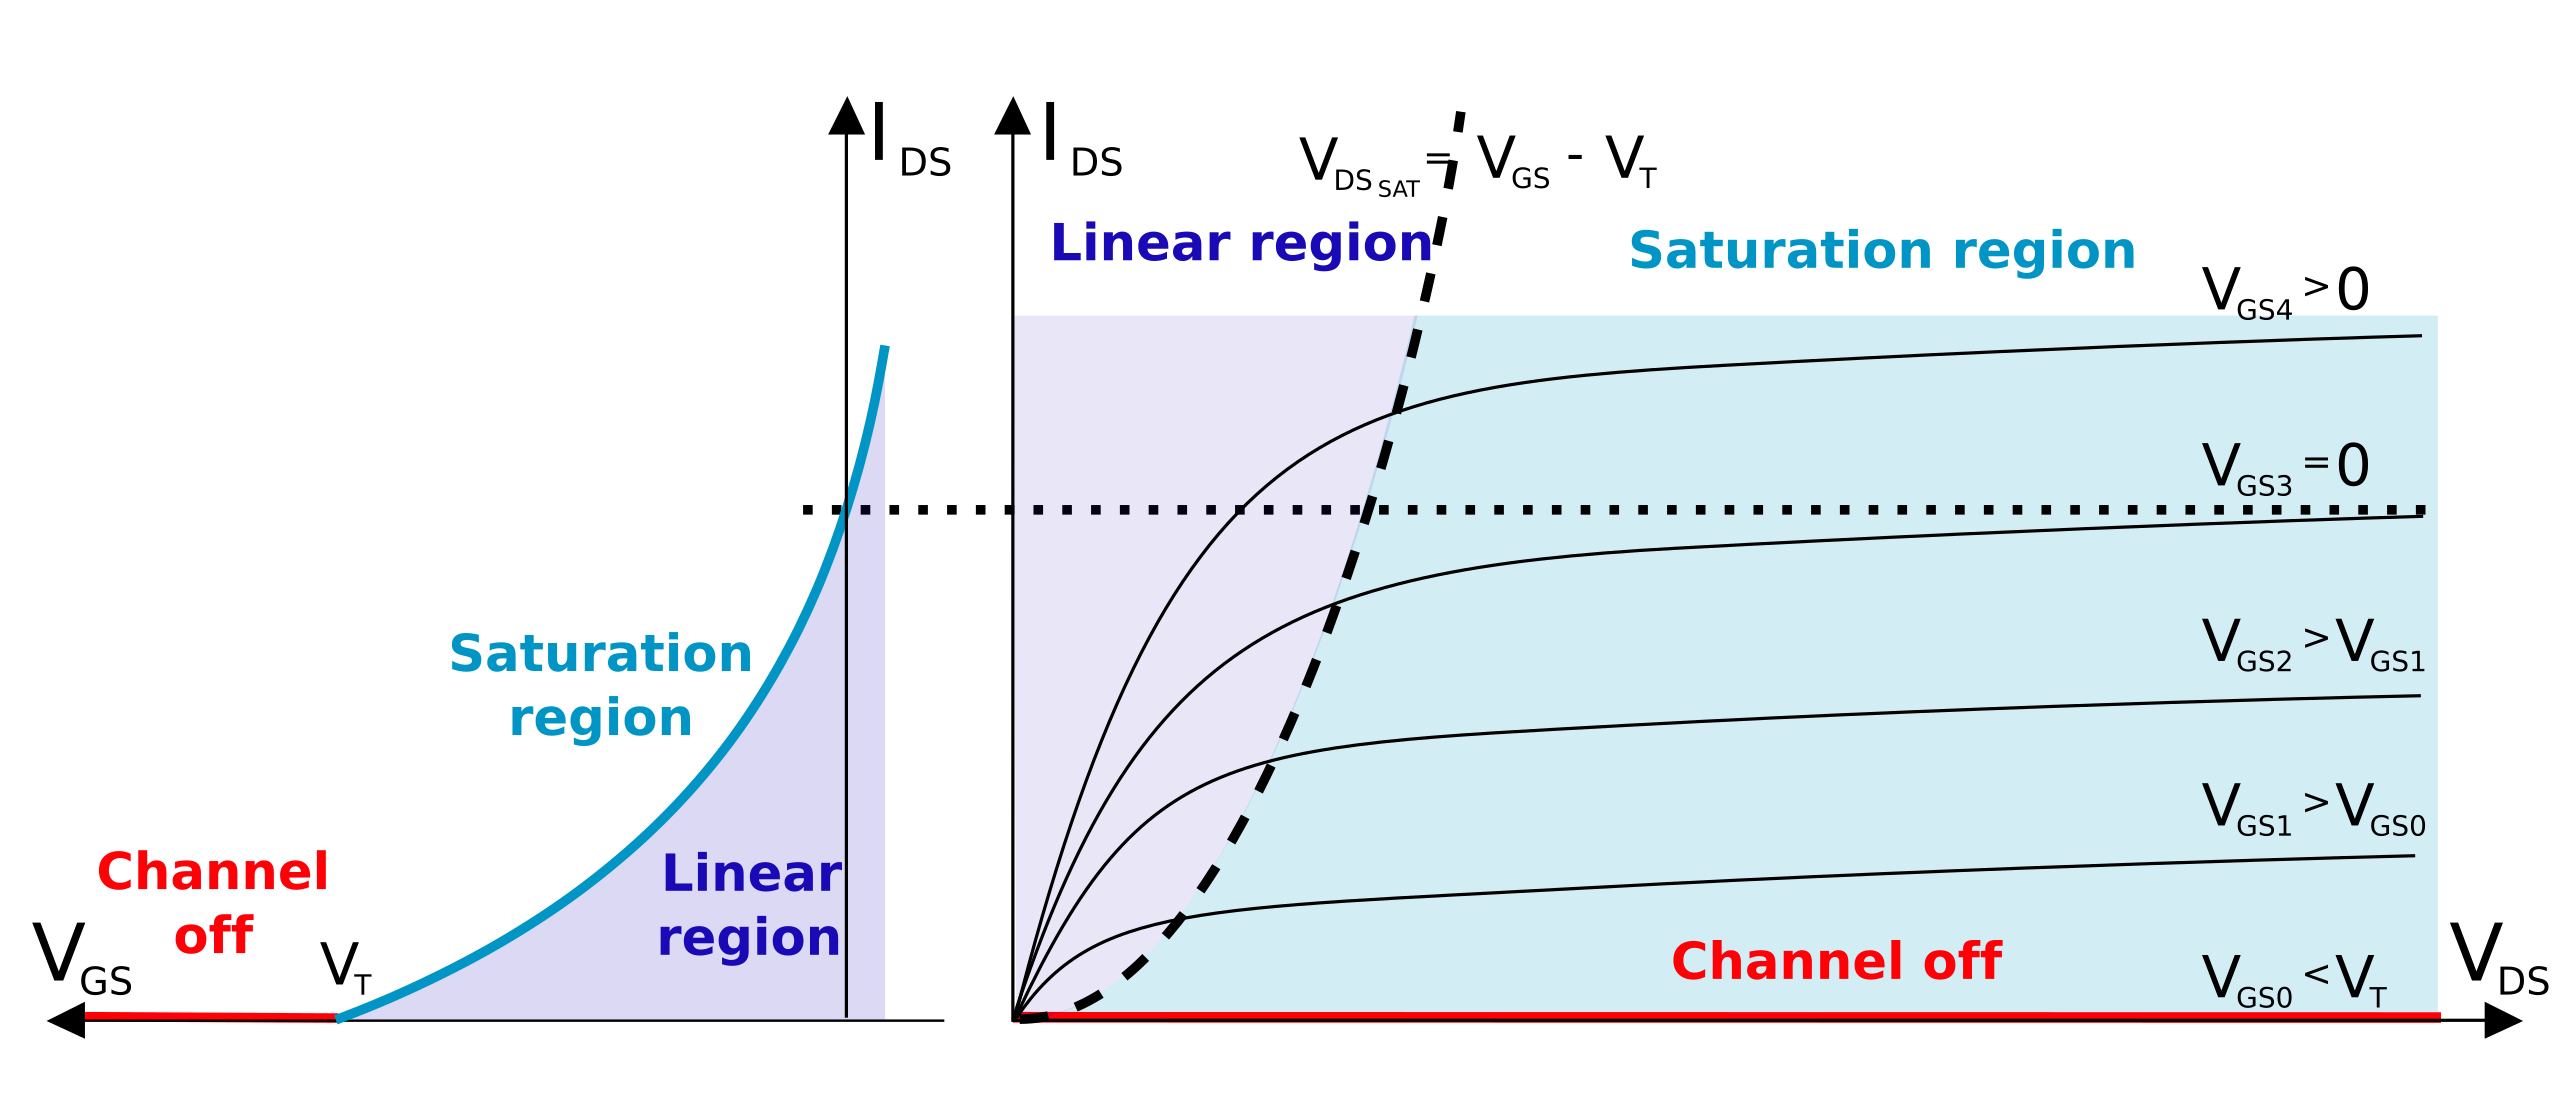
\includegraphics[width=0.65\linewidth,height=\textheight,keepaspectratio]{assets/imgs/caratteristiche_NMOS.png}
\caption{Curve caratteristiche di un transistor N-MOS.}
\end{figure}

Come accennato prima abbiamo a che fare con un generatore di corrente
\emph{governato in tensione}, in particolare dalla \(V_{DS}\), quella
tra drain e source. L'\emph{equazione della corrente (di Drain) è}: \[
i_{D}= \left\{ \begin{array}{cl}
K[2(V_{GS}-V_{T})V_{DS}-V^{2}_{DS})] & : \ V_{DS} \leq V_{GS} - V_{T} \\
i_{D-sat}=k(V_{GS}-V_{T}) & : \ V_{DS} \geq V_{GS} - V_{T}
\end{array} \right.
\] La prima equazione raffigura una \emph{parabola} che ha come
parametro la tensione \(V_{DS}\): avrà il proprio vertice in
\(V_{GS}-V_{T}\). La seconda equazione (che vale nel momento in cui
viene raggiunto il vertice della parabola) determina la corrente di
saturazione, e diventa una \textbf{costante}, con un coefficiente di
proporzionalità: \[
K=\frac{1}{2}\mu\:C_{ox}\frac{W}{L}
\] dove in \(K\), abbiamo più parametri: \(mu\) dovrebbe essere la
\emph{mobilità}\footnote{Quanto \emph{scorrono} facilmente le cariche al
  suo interno.} del materiale, \(C_{ox}\) la capacità dell'ossido per
unità di carica\footnote{Più è maggiore più ha possibilità di spostare
  cariche.}, mentre \(W\) rappresenta la larghezza della zona che va a
costituire il canale, mentre \(L\) è la lunghezza. \[
K\propto \mu \Rightarrow K_{n}\simeq 2K_{p}
\] All'aumentare della corrente il N-MOS si comporta come un resistore
la cui resistenza è data da
\(R=\frac{\rho\cdot L}{s}=\frac{\rho\cdot L}{W\cdot h}\). Posso quindi
riscrivere la costante: \[
K=\frac{h}{\rho}\cdot\frac{W}{L}
\] dove la prima parte rappresenta la parte ``tecnologica'', mentre la
seconda è la parte ``geometrica'' su cui posso agire per \emph{tarare}
la risposta di \(I_D\) rispetto a \(V_{DS}\). Inoltre la lunghezza \(L\)
determina la distanza tra Drain e Source e di conseguenza la lunghezza
del canale: questo è il parametro che va a determinare la tensione
massima tra Source e Drain prima di rompere il dispositivo. Questo
perché applicando una certa tensione \(V_{DS}\) la quale sviluppa un
campo elettrico e quanto sono più lontani i terminali quanto più basso è
il campo elettrico, e quindi il MOSFET potrà reggere tensioni più alte,
e viceversa.\newline Come nei BJT, una volta superata la cosiddetta
tensione di breakdown il dispositivo si rompe; questa tensione è
proporzionale al canale.

\begin{figure}
\centering
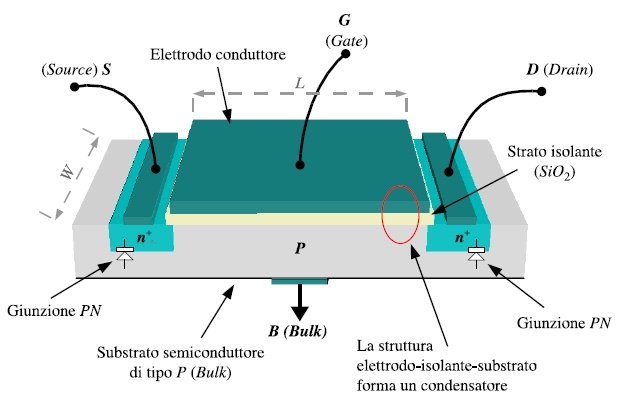
\includegraphics[width=0.5\linewidth,height=\textheight,keepaspectratio]{assets/imgs/nmos_dall_alto.png}
\caption{Vista di un transistor N-MOS dall'alto.}
\end{figure}

\subsection{P-MOS}\label{p-mos}

È il dispositivo \textbf{\emph{complementare all'N-MOS}}.

\begin{figure}[H]
\centering
\resizebox{0.7\textwidth}{!}{%
\begin{circuitikz}
\tikzstyle{every node}=[font=\LARGE]

\draw[thick, fill=blue!20]   (0,7.25) rectangle (11,3.25); %rettangolo principale
\draw[thick, fill=yellow!20]   (4,8.25) rectangle (7,7.25); %ossido
\draw[thick, fill=red!20]   (2,7.25) rectangle (4,6.25); %n+
\draw[thick, fill=red!60]   (4,9.25) rectangle (7,8.25); %metal gate
\draw[thick, fill=red!20]   (7,7.25) rectangle  node {\LARGE p+} (9,6.25);%n+
\node [font=\Large] at (5.5,5.25) {N};
\node [font=\Large] at (3,6.75) {p+};
\node [font=\Large] at (5.5,8.75) {Metal gate};
\node [font=\Large] at (5.5,7.75) {Ossido di S};
\node [font=\Large] at (3,8.5) {Source};
\draw [short] (3,8.25) -- (3,7.25);
\draw [short] (8,8.25) -- (8,7.25);
\node [font=\Large] at (8,8.5) {Gate};
\node [font=\Large] at (5.5,10.5) {Drain};
\draw [short] (5.5,10.25) -- (5.5,9.25);
\draw [<->, >=Stealth] (12,5.75) -- (15,5.75);
\draw  (4,9.25) rectangle (7,8.25);
\draw (18.75,7.5) to[Tpmos, transistors/scale=1.5] (18.75,4.5);
\draw  (19.25,6) circle (1.1cm);
\draw [->, >=Stealth] (20.75,6.75) .. controls (20.5,7.5) and (20.5,7.75) .. (19.75,7.75) node[pos=0.5,right, fill=white]{$V_{SG}$};
\draw (19.75,6) to[short] (20.5,6);
\draw [->, >=Stealth] (17.5,4.75) .. controls (17,6) and (17,6) .. (17.5,7) node[pos=0.5,left, fill=white]{$V_{SD}$};
\node [font=\large] at (18.75,7.75) {$S$};
\node [font=\large] at (20.75,6) {$G$};
\node [font=\large] at (18.75,4.25) {$D$};
\draw [->, >=Stealth] (18.25,8) -- (18.25,7)node[pos=0.5,left, fill=white]{I};
\draw [->, >=Stealth] (20.5,5.5) -- (21.25,5.5)node[pos=0.5,below, fill=white]{I};
\end{circuitikz}
}%

\label{fig:my_label}
\caption{Sezione di un transistor P-MOS}
\end{figure}

Valgono le stesse equazioni, ma le tensioni e le correnti sono
\emph{opposte} (\(V_{GS}<0,V_{DS}<0,V_{t}<0\)).\newline Applicando al
Ground una tensione negativa si accumulano cariche positive \emph{sotto
l'ossido}: si formerà dunque un canale di lacune. Il Drain sarà
considerato negativo rispetto al Source.

Il guadagno (e quindi la corrente di uscita) sono \emph{minori}, in
quanto le lacune sono portatori minoritari (come per i transistor BJT,
in quanto \(k_n\approx 2k_p\)), le quali andranno a formare il canale di
conduzione.

Le equazioni delle curve sono le stesse dell'N-MOS.

Per valutare K dato delle curve è possibile risolvere il seguente
sistema: \[
\begin{cases}
I_{D1}=K(V_{GS}-V_{t})^{2}\\
I_{D2}=K(V_{GS}-V_{t})^{2}\end{cases}\longrightarrow\begin{cases}\sqrt{I_{DS}}=\sqrt{K}(V_{GS}-V_{t})\\
\sqrt{I_{DS}}=\sqrt{K}(V_{GS}-V_{t})
\end{cases}
\]

\begin{bluebox}{Riepilogo dei transistor MOS}
I MOS hanno le seguenti regioni:
\begin{enumerate}
\item Quando la tensione di Gate è inferiore alla tensione di soglia ($V_{G}<V_{th}$ entrambe in valore assoluto), siamo in \emph{cutoff}: non abbiamo portatori nel canale. Siamo in interdizione ed il dispositivo è spento e non passa corrente tra source e drain;
\item Nella regione \emph{lineare}, in cui ci troviamo superando la tensione di soglia per piccole tensioni di drain, la (curva) caratteristica della corrente è \emph{parabolica}: inizialmente si potrebbe approssimare con una retta (da qui lineare). La pendenza di quest'ultima mi indica la resistenza del canale, tant'è che il dispositivo viene detto \emph{\textbf{resistore controllato in tensione}} (di Gate)! Sono inversamente proporzionali.
\item Una volta raggiunto il vertice della parabola ci troviamo nella regione detta \emph{di saturazione} la corrente diventa \textbf{costante} e sempre dipendente dalla tensione di Gate: il transistor è un generatore di corrente controllato in tensione.
\end{enumerate}
\end{bluebox}

\subsection{Real N-MOS}\label{real-n-mos}

All'apparenza il transistor N-MOS sembra un dispositivo
\emph{simmetrico}, ma non lo è. Infatti in precedenza abbiamo assunto la
tensione \(V_{DS}>0\) perché polarizzando la S viene polarizzato anche
il blocco P\footnote{O \(n\) se in un P-MOS.} sottostante: in questo
modo si viene a formare un \textbf{\emph{body diode}} tra l'emettitore
ed il collettore. In sostanza si va a \emph{cortocircuitare} (viene
metallizzato) Source con la regione di tipo P: rimane la giunzione tra P
e il Drain.

\begin{redbox}{Body diode} 
Il \textbf{body diode} (o di bulk) sono diodi \textbf{\emph{intrinseci}} per qualsiasi transistor ad effetto di campo. Nelle applicazioni FET a canale N, la corrente scorre tipicamente dal drain alla source a causa della polarità del body diode. Anche se non è stato indotto un canale, la corrente può comunque fluire dalla source al drain attraverso la connessione in cortocircuito source-body e il diodo body-drain. Per questo motivo, un tipico FET a canale N non può bloccare il flusso di corrente dalla sorgente al drain.
\end{redbox}

Nel nostro caso è essenzialmente una giunzione p-n \emph{parassita} in
cui passa la corrente invece che nel canale.

\begin{figure}[h!]
  \centering
  \begin{minipage}{0.45\textwidth}
    \centering
    \resizebox{0.6\textwidth}{!}{ % Ridimensiona la figura al 80% della larghezza
      \begin{circuitikz}
        \tikzstyle{every node}=[font=\LARGE]
        \draw  (1,7.25) rectangle (10,3.25);
        \draw  (4,8.25) rectangle (7,7.25);
        \draw  (2,7.25) rectangle (4,6.25);
        \draw  (7,7.25) rectangle  node {\LARGE n+} (9,6.25);
        \node [font=\Large] at (5.5,5.25) {P};
        \node [font=\Large] at (3,6.75) {n+};
        \node [font=\Large] at (5.5,8.75) {Metal gate};
        \node [font=\Large] at (5.5,7.75) {Ossido di S};
        \node [font=\Large] at (3,8.5) {Source};
        \draw [short] (3,8.25) -- (3,7.25);
        \draw [short] (8,8.25) -- (8,7.25);
        \node [font=\Large] at (8,8.5) {Gate};
        \draw [short] (5.5,10.25) -- (5.5,9.25);
        \node [font=\Large] at (5.5,10.5) {Drain};
        \draw  (4,9.25) rectangle (7,8.25);
        \draw (5.5,3.25) to[D] (8,6.25);
      \end{circuitikz}
    }
    \caption{Presenza nel real N-MOS del body diode}
  \end{minipage}
  \hspace{1cm}
  \begin{minipage}{0.45\textwidth}
    \centering
    \begin{circuitikz}
      \draw (0,0) node[nigfete](M1){};
      \draw (M1.G) -- (-1,0) node[left]{Gate};
      \draw (M1.D) -- (0,1.2) node[above]{Drain};
      \draw (M1.S) -- (0,-1.2) node[below]{Source};
      \draw (1,-1) to[diode] (1,1);
      \draw (0,-1) to[short] (1,-1);
      \draw (0,1) to[short] (1,1);
    \end{circuitikz}
    \caption{Schema circuitale del real N-MOS}
  \end{minipage}
\end{figure}

Se \(V_{DS}<0\) il diodo in questione è in \emph{forward bias}, e la
corrente \(i_D\) non dipende più dal gate\footnote{Nel transistore P-MOS
  accade se la tensione tra drain e source \(V_{DS}>0\)}: non abbiamo
quindi più il controllo sul dispositivo, perché la corrente scorre nel
diodo indipendentemente dalla tensione applicata sul Gate. Per evitarlo
la tensione di Drain dovrebbe essere maggiore rispetto a quella di
Source.

Il P-MOS reale funziona al contrario.

\chapter{Digital Logic Circuits (circuiti a logica
digitale)}\label{digital-logic-circuits-circuiti-a-logica-digitale}

Servono per trasferire e processare informazioni tra dispositivi
\textbf{senza modificare i valori}, funzionano realizzando operazioni
\emph{booleane} su dati booleani.

\section{Famiglie logiche}\label{famiglie-logiche}

\begin{redbox}{Definizione: famiglie logiche}
Una \textbf{famiglia logica} è un insieme di dispositivi elettronici i quali, se connessi tra di loro in modo opportuno, permettono di realizzare una qualsiasi funzione logica. Queste sono funzioni che definiscono lo stato di un'uscita per ogni possibile configurazione degli stati.
\end{redbox}

\subsection{Operatori logici
(booleani)}\label{operatori-logici-booleani}

\begin{itemize}
\tightlist
\item
  \textbf{NOT} (negazione): restituisce il bit negato.
\end{itemize}

\begin{figure}[h!]
  \centering
  \begin{minipage}{0.45\textwidth}
    \centering
    % Porta NOT con A e $\overline{A}$
    \begin{circuitikz}
      \node [not port](O1) at (0,0) {};    % Porta NOT
      \node at (-1, 0) {A};                 
      \node at (1, 0) {$\overline{A}$};     
    \end{circuitikz}
    \caption{Simbolo circuitale di NOT con A e $\overline{A}$}
  \end{minipage}%
  \hspace{0.5cm} % Spazio tra le due sottofigure
  \begin{minipage}{0.45\textwidth}
    \centering
    % Tabella di verità per NOT senza l'ambiente table
    \begin{tabular}{l|l}
      A & $\overline{A}$ \\ \hline
      0 & 1              \\
      1 & 0             
    \end{tabular}
    \caption{Tabella di verità per NOT}
  \end{minipage}
\end{figure}

\begin{itemize}
\tightlist
\item
  \textbf{AND} (prodotto logico): restituisce vero se \emph{entrambi i
  bit sono veri}.
\end{itemize}

\begin{figure}[h!]
  \centering
  \begin{minipage}{0.45\textwidth}
    \centering
    % Porta AND con A e B
    \begin{circuitikz}
      \node [and port](O1) at (0,0) {};    % Porta AND
      \node at (-2, 0.25) {A};                % A a sinistra
      \node at (-2, -0.3) {B};                 % B a destra
      \node at (0.75, 0) {A$\cdot$B};                 % B a destra
    \end{circuitikz}
    \caption{Simbolo circuitale di AND con A e B}
  \end{minipage}%
  \hspace{0.5cm} % Spazio tra le due sottofigure
  \begin{minipage}{0.45\textwidth}
    \centering
    % Tabella di verità per AND
    \begin{tabular}{c|c|c}
    A & B & A+B  \\ 
    \hline
    0 & 0 & 0    \\
    1 & 0 & 0    \\
    0 & 1 & 0    \\
    1 & 1 & 1   
    \end{tabular}
    \caption{Tabella di verità per AND}
  \end{minipage}
\end{figure}

\begin{itemize}
\tightlist
\item
  \textbf{OR} (somma logica): restituisce vero se \emph{almeno un bit è
  vero}.
\end{itemize}

\begin{figure}[h!]
  \centering
  \begin{minipage}{0.45\textwidth}
    \centering
    % Porta AND con A e B
    \begin{circuitikz}
      \node [or port](O1) at (0,0) {};    % Porta OR
      \node at (-2, 0.25) {A};                % A a sinistra
      \node at (-2, -0.3) {B};                 % B a destra
      \node at (0.75, 0) {A+B};                 % B a destra
    \end{circuitikz}
    \caption{Simbolo circuitale di AND con A e B}
  \end{minipage}%
  \hspace{0.5cm} % Spazio tra le due sottofigure
  \begin{minipage}{0.45\textwidth}
    \centering
    % Tabella di verità per AND
    \begin{tabular}{c|c|c}
    A & B & A+B  \\ 
    \hline
    0 & 0 & 0    \\
    1 & 0 & 1    \\
    0 & 1 & 1    \\
    1 & 1 & 1   
    \end{tabular}
    \caption{Tabella di verità per AND}
  \end{minipage}
\end{figure}

Concatenando queste porte logiche è possibile costruire una
\emph{qualsiasi operazione logica complessa}.

\subsection{Leggi (o teoremi) di de
Morgan}\label{leggi-o-teoremi-di-de-morgan}

Servono a stabilire relazioni di equivalenza tra la congiunzione (AND) e
la disgiunzione (OR) logica: attraverso la negazione (NOT) è possibile
esprimere queste due porte logiche in \emph{termini reciproci}. Le leggi
sono le seguenti \begin{align*}
\tag{1}A+B=\overline{\overline{A}\cdot\overline{B}}&\Longrightarrow \overline{A+B}=\overline{A}\cdot\overline{B} \\
\tag{2}A\cdot B=\overline{\overline{A}+\overline{B}}&\Longrightarrow\overline{A\cdot B}=\overline{A}+\overline{B}
\end{align*} A parole:

\begin{itemize}
\tightlist
\item
  La legge \((1)\) dice che effettuare la negazione dell'operazione di
  AND tra due ingressi equivale all'OR tra la negazione dei due singoli
  ingressi;
\item
  Allo stesso modo la legge numero \((2)\) ci dice che la negazione
  dell'operazione OR tra i due ingressi equivale alla somma tra gli
  stessi ingressi negati singolarmente.
\end{itemize}

A questo punto possiamo ricavare due porte:

\begin{itemize}
\tightlist
\item
  \textbf{NAND}: o ``NOT AND'', è un dispositivo complementare alla
  porta AND. Per le leggi di Morgan un NAND equivale all'operazione di
  OR tra due ingressi negati.

  \begin{figure}[h!]
  \centering
  \begin{minipage}{0.45\textwidth}
    \centering
    % Porta NAND con A e B
    \begin{circuitikz}
      \node [nand port](O1) at (0,0) {};    % Porta NAND
      \node at (-2, 0.25) {A};                % A a sinistra
      \node at (-2, -0.3) {B};                % B a destra
      \node at (0.75, 0) {$\overline{A\cdot B}$}; % Etichetta per NAND
    \end{circuitikz}
    \caption{Simbolo circuitale di NAND con A e B}
  \end{minipage}%
  \hspace{0.5cm} % Spazio tra le due sottofigure
  \begin{minipage}{0.45\textwidth}
    \centering
    % Tabella di verità per NAND
    \begin{tabular}{c|c|c|c|c|c}
    A & B & $\overline{A}$ & $\overline{B}$ & A $\cdot$ B & $\overline{A\cdot B}$ \\ 
    \hline
    0 & 0 & 1 & 1 & 0 & 1    \\
    1 & 0 & 0 & 1 & 0 & 1    \\
    0 & 1 & 1 & 0 & 0 & 1    \\
    1 & 1 & 0 & 0 & 1 & 0   
    \end{tabular}
    \caption{Tabella di verità per NAND}
  \end{minipage}
  \end{figure}
\item
  \textbf{NOR}: o ``NOT OR'', è il dispositivo complementare alla porta
  OR. Sempre per le leggi di Morgan un NOR equivale all'operazione AND
  fra due ingressi negati
\end{itemize}

\begin{figure}[h!]
  \centering
  \begin{minipage}{0.45\textwidth}
    \centering
    % Porta NOR con A e B
    \begin{circuitikz}
      \node [nor port](O1) at (0,0) {};    % Porta NOR
      \node at (-2, 0.25) {A};                % A a sinistra
      \node at (-2, -0.3) {B};                % B a destra
      \node at (0.75, 0) {A + B};             % Etichetta per NOR
    \end{circuitikz}
    \caption{Simbolo circuitale di NOR con A e B}
  \end{minipage}%
  \hspace{0.5cm} % Spazio tra le due sottofigure
  \begin{minipage}{0.45\textwidth}
    \centering
    % Tabella di verità per NOR con A, B, A negato, B negato, A AND B e A NOR B
    \begin{tabular}{c|c|c|c|c|c}
    A & B & $\overline{A}$ & $\overline{B}$ & A + B & $\overline{A + B}$ \\ 
    \hline
    0 & 0 & 1 & 1 & 0 & 1    \\
    1 & 0 & 0 & 1 & 1 & 0    \\
    0 & 1 & 1 & 0 & 1 & 0    \\
    1 & 1 & 0 & 0 & 1 & 0   
    \end{tabular}
    \caption{Tabella di verità per NOR}
  \end{minipage}
\end{figure}
\begin{bluebox}{Osservazione: \emph{completezza} della famiglia logica}
Una famiglia logica si dice \emph{\textbf{completa}} quando tra i suoi dispositivi è presente la porta NOT ed una tra la porta AND o la porta OR. In particolare è possibile realizzare, con le porte NAND e NOR, tutte le porte precedenti: in questo modo quindi \emph{\textbf{si possono realizzare tutti i circuiti con una singola porta!}}
\end{bluebox}

\begin{itemize}
\tightlist
\item
  Esempi:

  \begin{figure}[H]
  \centering
  \begin{subfigure}{0.45\textwidth}
  \centering
  \resizebox{\textwidth}{!}{%
  \begin{circuitikz}
  \tikzstyle{every node}=[font=\large]
  \draw (4,15) to[short] (4.75,15);
  \draw (4,14.5) to[short] (4.75,14.5);
  \draw (4.75,15) node[ieeestd nand port, anchor=in 1, scale=0.89](port){} (port.out) to[short] (7,14.75);
  \draw (4,15) to[short] (3,15);
  \draw (3.5,15) to[short] (3.5,14.5);
  \draw (3.5,14.5) to[short] (4,14.5);
  \node [font=\large] at (2.5,15) {$A$};
  \node [font=\large] at (8,14.75) {$\overline{A \cdot A} = \overline{A}$};
  \end{circuitikz}
  }
  \caption{Porta NOT con NAND}
  \label{not_nand}
  \end{subfigure}
  \hfill
  \begin{subfigure}{0.45\textwidth}
  \centering
  \resizebox{\textwidth}{!}{%
  \begin{circuitikz}
  \tikzstyle{every node}=[font=\large]
  \draw (4,15) to[short] (4.75,15);
  \draw (4,14.5) to[short] (4.75,14.5);
  \draw (4.75,15) node[ieeestd nor port, anchor=in 1, scale=0.89](port){} (port.out) to[short] (7,14.75);
  \draw (4,15) to[short] (3,15);
  \draw (3.5,15) to[short] (3.5,14.5);
  \draw (3.5,14.5) to[short] (4,14.5);
  \node [font=\large] at (2.5,15) {$A$};
  \node [font=\large] at (8,14.75) {$\overline{A + A} = \overline{A}$};
  \end{circuitikz}
  }
  \caption{Porta NOT con NOR}
  \label{not_nor}
  \end{subfigure}
  \caption{Rappresentazioni della porta NOT.}
  \label{fig:not}
  \end{figure}
\end{itemize}

\begin{figure}[H]
\centering
\begin{subfigure}{0.45\textwidth}
\centering
\resizebox{\textwidth}{!}{%
\begin{circuitikz}
\tikzstyle{every node}=[font=\normalsize]
\draw (1,19.25) to[short] (1.25,19.25);
\draw (1,18.75) to[short] (1.25,18.75);
\draw (1.25,19.25) node[ieeestd nand port, anchor=in 1, scale=0.89](port){} (port.out) to[short] (3,19);
\draw (3,19) to[short] (4,19);
\draw (5,19.25) to[short] (5.25,19.25);
\node [font=\normalsize] at (3.75,19.2) {$A\cdot B$};
\draw (5,18.75) to[short] (5.25,18.75);
\draw (5.25,19.25) node[ieeestd nand port, anchor=in 1, scale=0.89](port){} (port.out) to[short] (7,19);
\draw (4.5,19.25) to[short] (5,19.25);
\draw (4.5,18.75) to[short] (5,18.75);
\draw (4,19) to[short] (4.5,19);
\draw (4.5,18.75) to[short] (4.5,19.25);
\node [font=\normalsize] at (0.75,19.25) {A};
\node [font=\normalsize] at (0.75,18.75) {B};
\node [font=\normalsize] at (9.5,19) {$\overline{\overline{AB} \cdot \overline{AB}} = AB + AB = AB$};
\end{circuitikz}
}
\caption{Porta AND con NAND}
\label{and_nand}
\end{subfigure}
\hfill
\begin{subfigure}{0.45\textwidth}
\centering
\resizebox{\textwidth}{!}{%
\begin{circuitikz}
\tikzstyle{every node}=[font=\normalsize]

\draw (0,32.5) to[short] (0.25,32.5);
\draw (0,32) to[short] (0.25,32);
\draw (0.25,32.5) node[ieeestd nor port, anchor=in 1, scale=0.89](port){} (port.out) to[short] (2,32.25);
\draw (0,30.5) to[short] (0.25,30.5);
\draw (0,30) to[short] (0.25,30);
\draw (0.25,30.5) node[ieeestd nor port, anchor=in 1, scale=0.89](port){} (port.out) to[short] (2,30.25);
\draw (-1,32.5) to[short] (0,32.5);
\draw (-0.5,32.5) to[short] (-0.5,32);
\draw (-0.5,32) to[short] (0,32);
\draw (-1,30.5) to[short] (0,30.5);
\draw (-0.5,30.5) to[short] (-0.5,30);
\draw (-0.5,30) to[short] (0,30);
\draw (3,31.5) to[short] (3.25,31.5);
\draw (3,31) to[short] (3.25,31);
\draw (3.25,31.5) node[ieeestd nor port, anchor=in 1, scale=0.89](port){} (port.out) to[short] (5,31.25);
\draw (2,32.25) to[short] (2.5,32.25);
\draw (2.5,32.25) to[short] (2.5,31.5);
\draw (2.5,31.5) to[short] (3,31.5);
\draw (2,30.25) to[short] (2.5,30.25);
\draw (2.5,31) to[short] (2.5,30.25);
\draw (2.5,31) to[short] (3,31);
\node [font=\normalsize] at (-1.2,32.5) {A};
\node [font=\normalsize] at (-1.2,30.5) {B};
\node [font=\normalsize] at (3,31.75) {$\overline{A}$};
\node [font=\normalsize] at (3,30.75) {$\overline{B}$};
\node [font=\normalsize] at (6.5,31.25) {$\overline{(\overline{A}+\overline{B})}=A\cdot B$};
\end{circuitikz}
}
\caption{Porta AND con NOR}
\label{and_nor}
\end{subfigure}
\caption{Rappresentazioni della porta AND.}
\label{fig:and}
\end{figure}
\begin{figure}[H]
\centering
\begin{subfigure}{0.45\textwidth}
\centering
\resizebox{\textwidth}{!}{%
\begin{circuitikz}
\tikzstyle{every node}=[font=\normalsize]
\draw (0,34.5) to[short] (0.25,34.5);
\draw (0,34) to[short] (0.25,34);
\draw (0.25,34.5) node[ieeestd nand port, anchor=in 1, scale=0.89](port){} (port.out) to[short] (2,34.25);
\draw (0,32.5) to[short] (0.25,32.5);
\draw (0,32) to[short] (0.25,32);
\draw (0.25,32.5) node[ieeestd nand port, anchor=in 1, scale=0.89](port){} (port.out) to[short] (2,32.25);
\draw (3,33.5) to[short] (3.25,33.5);
\draw (3,33) to[short] (3.25,33);
\draw (3.25,33.5) node[ieeestd nand port, anchor=in 1, scale=0.89](port){} (port.out) to[short] (5,33.25);
\draw (2,34.25) to[short] (2.5,34.25);
\draw (2.5,34.25) to[short] (2.5,33.5);
\draw (2.5,33.5) to[short] (3,33.5);
\draw (2,32.25) to[short] (2.5,32.25);
\draw (2.5,33) to[short] (2.5,32.25);
\draw (2.5,33) to[short] (3,33);
\draw (-0.5,34.5) to[short] (0.25,34.5);
\draw (-0.25,34.5) to[short] (-0.25,34);
\draw (-0.25,34) to[short] (0.25,34);
\draw (-0.5,32.5) to[short] (0,32.5);
\draw (-0.25,32.5) to[short] (-0.25,32);
\draw (-0.25,32) to[short] (0.25,32);
\node [font=\normalsize] at (-0.75,34.5) {$A$};
\node [font=\normalsize] at (-0.75,32.5) {$B$};
\node [font=\normalsize] at (2.25,34.5) {$\overline{A}$};
\node [font=\normalsize] at (2.25,32) {$\overline{B}$};
\node [font=\normalsize] at (6.5,33.25) {$\overline{\overline{A}\cdot\overline{B}}=A+B$};
\end{circuitikz}
}
\caption{Porta OR con NAND}
\label{or_nand}
\end{subfigure}
\hfill
\begin{subfigure}{0.45\textwidth}
\centering
\resizebox{\textwidth}{!}{%
\begin{circuitikz}
\tikzstyle{every node}=[font=\normalsize]
\draw (1,3.5) to[short] (1.25,3.5);
\draw (1,3) to[short] (1.25,3);
\draw (1.25,3.5) node[ieeestd nor port, anchor=in 1, scale=0.89](port){} (port.out) to[short] (3,3.25);
\draw (5,3.5) to[short] (5.25,3.5);
\draw (5,3) to[short] (5.25,3);
\draw (5.25,3.5) node[ieeestd nor port, anchor=in 1, scale=0.89](port){} (port.out) to[short] (7,3.25);
\draw (3,3.25) to[short] (4,3.25);
\draw (4,3.25) to[short] (4.5,3.25);
\draw (5,3) to[short] (4.5,3);
\draw (4.5,3) to[short] (4.5,3.5);
\draw (4.5,3.5) to[short] (5,3.5);
\node [font=\normalsize] at (0.75,3.75) {$A$};
\node [font=\normalsize] at (0.75,3) {$B$};
\node [font=\normalsize] at (3.75,3.5) {$\overline{A+B}$};
\node [font=\normalsize] at (9.4,3.25) {$(\overline{\overline{A}+\overline{B}})=\overline{\overline{A+B}}=A+B$};
\end{circuitikz}
}
\caption{Porta OR con NOR}
\label{or_nor}
\end{subfigure}
\caption{Rappresentazioni della porta OR.}
\label{fig:or}
\end{figure}

In elettronica, lo stato logico \(0\) è associato ad una \emph{bassa
tensione}, mentre lo stato \(1\) è associato ad un'\emph{alta tensione}.

\section{Famiglie logiche: parametri
statici}\label{famiglie-logiche-parametri-statici}

Quando si tratta un segnale logico, ci si aspetta che esso sia
\textbf{\emph{ben definito}}: in particolare deve essere ben chiaro
quando il segnale è ``alto'' e quando è basso. Per ogni famiglia logica
quindi esistono quindi una serie di parametri che ne definiscono il
funzionamento. I seguenti parametri sono detti statici in quanto sono
misurati con il circuito ``fermo'', senza commutazioni: non dipendono
dal fatto che il segnale stia variando nel tempo.

\begin{enumerate}
\def\labelenumi{\arabic{enumi})}
\tightlist
\item
  \textbf{Tensione di ingresso}: discrimina il valore \emph{logico} in
  base alla tensione d'ingresso, quindi come questa sia
  \emph{interpretata}:

  \begin{itemize}
  \tightlist
  \item
    \(V_{iL} \doteq\) è il \textbf{massimo} valore di tensione in
    ingresso che la famiglia logica rileva come \emph{livello logico
    basso} (oppure \(0\) logico, stato negativo);
  \item
    \(V_{iH} \doteq\) è il \textbf{minimo} valore di tensione in
    ingresso che la famiglia logica (o l'integrato) percepisce come
    \emph{livello logico alto} (oppure \(1\) logico, stato positivo).
  \end{itemize}
\item
  \textbf{Tensione di uscita}: indica come interpretare i valori
  rilevati all'uscita di un circuito:

  \begin{itemize}
  \tightlist
  \item
    \(V_{oL} \doteq\) è il \textbf{massimo} valore della tensione in
    uscita da una porta logica\footnote{La porta successiva potrà
      riconoscerlo.} dalla porta logica tale che, in base alle
    specifiche del prodotto, corrisponde ad un livello logico
    \textbf{basso} (\(0\) logico);
  \item
    \(V_{oH} \doteq\) è il \textbf{minimo} valore della tensione in
    uscita da una porta logica che in base alle specifiche del prodotto
    stabilisce un valore logico \textbf{alto} (\(1\) logico).
  \end{itemize}
\end{enumerate}

\begin{orangebox}{Nota: Regione di indeterminazione.}
Per evitare ambiguità devono valere:
$$
V_{iL}\leq V_{iH}; \quad V_{oL}\leq V_{oH}
$$
Idealmente tutti i valori in ingresso \emph{corrispondono} ai valori in uscita. Tuttavia questo non è possibile, a causa di possibili variazioni ambientali e/o nel processo di costruzione. Si usano quindi dei valori $V_{i/o L}$ più bassi dei $V_{i/oH}$, statisticamente \emph{certi}, i quali considerano anche le possibili oscillazioni dei valori. Questo perché rispettando questi valori definiti del costruttore del circuito in tutte le condizioni operative il segnale sarà interpretato/percepito \textbf{correttamente}. \newline
Infatti sappiamo che un qualsiasi valore di tensione di ingresso compreso tra $\left[\mathrm{V}_{\mathrm{iL-max}},\mathrm{V}_{\mathrm{iH-min}}\right]$ non sappiamo quando potrà essere riconosciuto dalla porta come 1 logico o come 0 logico: si dice che sono valori nella \emph{\textbf{regione di indeterminazione}}. Inoltre, per una far sì che non ci siano errori di interpretazione è necessario che l'operazione di commutazione tra gli stati sia il più \emph{veloce} possibile, in quanto il valore in questi casi passa nella regione.\newline Allo stesso modo, un qualsiasi valore di tensione di uscita compreso nell'intervallo $[\mathrm{V}_{\mathrm{oL-max}},\mathrm{V}_{\mathrm{oH-min}}]$ non potrà essere riconosciuto con 1 logico o come 0 logico da una porta posta immediatamente in cascata.
\begin{minipage}{\linewidth}
\centering
\resizebox{0.3\textwidth}{!}{%
\begin{circuitikz}
\tikzstyle{every node}=[font=\small]
% Disegna le linee orizzontali
\draw [short] (0,2) -- (4,2);
\draw [short] (0,0) -- (4,0);
% Colora la zona tra le due linee orizzontali
\fill[blue, opacity=0.2] (0,0) rectangle (4,2);
% Aggiungi le etichette
\node [font=\footnotesize] at (2,1) {\textit{Regione di Indeterminazione}};
\node [font=\normalsize] at (4.5,2) {$V_{iH}$};
\node [font=\normalsize] at (4.5,0) {$V_{iL}$};
\end{circuitikz}
}%
\end{minipage}
\end{orangebox}

\begin{enumerate}
\def\labelenumi{\arabic{enumi})}
\setcounter{enumi}{2}
\tightlist
\item
  \textbf{Corrente assorbita}:

  \begin{itemize}
  \tightlist
  \item
    \(I_{iH}\): corrente assorbita in ingresso quando viene applicato il
    valore logico alto;
  \item
    \(I_{iL}\): corrente assorbita in ingresso quando viene applicato il
    valore logico basso.
  \end{itemize}
\end{enumerate}

Da queste grandezze ne derivano altre 3:

\begin{enumerate}
\def\labelenumi{\arabic{enumi})}
\setcounter{enumi}{3}
\tightlist
\item
  \textbf{Noise Margin}\footnote{Più è alto meglio è; \emph{higher
    better}.}: resilienza del circuito al rumore; quanto disturbo può
  ricevere \emph{senza influire sul suo comportamento}. È la quantità
  cui il segnale eccede la soglia minima \(V_{iH}\) e \(V_{iL}\): \[
   NM=\min(NM_{H}, NM_{L}); \quad NM_{H}=V_{oH}-V_{iH}; \quad NM_{L}=V_{iL}-V_{oL}
   \]

  \begin{bluebox}{Osservazione}
  $NM_{H}$ e $NM_{L}$ devono essere \textbf{positivi}, per cui è necessario che le tensioni siano:
  $$
  V_{oH}>V_{iH};\quad V_{iL}>V_{oL}
  $$
  Maggiore è la differenza tra i valori (e quindi il Noise Margin), maggiore è il grado di "certezza" dell'interpretazione del segnale.
  \end{bluebox}
\item
  \textbf{Fan-out}\footnote{Più è alto meglio è; \emph{higher better}.}:
  rappresenta il \textbf{\emph{massimo numero di porte d'ingresso}} che
  posso guidare/pilotare (collegabili ad un'uscita) mantenendo un valore
  logico \emph{corretto} (dipende da \(I_{i\:L},\:I_{i\:H}\));
\item
  \textbf{Static power}\footnote{Più bassa è meglio è; lower better.}:
  rappresenta la \textbf{\emph{potenza assorbita (o dissipata) in
  condizioni statiche}}. È pari alla media tra le potenze assorbite con
  un'uscita alta/bassa; \[
   P=\frac{(P_{H}+P_{L})}{2}
   \] dove \(P_H = V_{cc}\cdot i_H\) e \(P_L=V_{cc}\cdot i_L\).
\end{enumerate}

\section{\texorpdfstring{Famiglie logiche: parametri
\emph{dinamici}.}{Famiglie logiche: parametri dinamici.}}\label{famiglie-logiche-parametri-dinamici.}

I parametri precedenti devono essere misurati in condizioni
\emph{statiche}, mentre questi si misurano \textbf{\emph{al momento di
una commutazione di stato}}\footnote{Quindi la porta logica cambia dallo
  stato alto al basso o viceversa.}.

\begin{enumerate}
\def\labelenumi{\arabic{enumi})}
\tightlist
\item
  \textbf{Ritardo/tempo di propagazione} (propagation delay): indicato
  con \(t_{p_{HL}}\) e \(t_{p_{LH}}\), rappresenta in quanto tempo un
  cambio in ingresso è \emph{percepito} (e riportato) dall'uscita. È
  fondamentale che sia \textbf{basso}: ad esempio con \(10\:ns\) siamo
  vincolati a processi con frequenza massima di \(100\) MHz; tra i due
  tempi di propagazione conta quello \textbf{più lento}, ovvero quello
  più penalizzante.
\item
  \textbf{Energia di commutazione} (Switching power): indica l'energia
  impiegata (in Joule) per commutare uno stato, essa cresce
  \emph{linearmente} con la velocità del circuito (lower better). Viene
  integrata per il tempo della commutazione;
\item
  \textbf{Prodotto ritardo-potenza} (Delay-Power product): è il prodotto
  tra il ritardo di propagazione e la potenza dissipata nel circuito;
  serve per \emph{bilanciare} le prime due, le quali sono tra loro
  discordi (lower better). A livello del design del circuito si può
  aumentare la potenza e di conseguenza diminuirà il ritardo di
  propagazione (a parità di circuito). La potenza dipende dalle
  resistenze, mentre il ritardo dalle capacità.
\end{enumerate}

\section{RTL (Resistor-Transistor
Logic)}\label{rtl-resistor-transistor-logic}

È una famiglia di porte logiche \emph{che usano i transistor BJT} e
resistenze per realizzare le porte. Il sistema è obsoleto a causa del
suo fan-in limitato (al massimo 3 ingressi). Alcuni esempi di porte
sono:

\begin{itemize}
\tightlist
\item
  \textbf{NOT}: Corrisponde ad un transistor con una resistenza di base
  \(R_B\) e una resistenza di collettore \(R_C\), l'ingresso è collegato
  alla base del transistor; il dispositivo si comporta come un
  \emph{invertitore}. In questa configurazione, ovvero quando
  l'emettitore è collegato a massa, si parla di emettitore comune.
\end{itemize}

\begin{figure}[H]
\centering
\resizebox{0.5\textwidth}{!}{%
\begin{circuitikz}[american]
    % Resistor RB
    \draw node[american not port] at (1, 5) {};
    \draw [R=,a={$R_B$}, l={$450\:\Omega$}] (6, 5) to (3, 5);
    % Ground node
    \draw node[ground] (N1) at (7, 2.75) {} node[anchor=south west] at (N1.north east) {$0$};
    % Transistor Q1
    \draw node[npn] (N2) at (7, 5) {} node[anchor=south east] at ([xshift=0.56cm, yshift=-0.56cm]N2.north west) {$Q1$};
    % Connect the nodes
    \draw (6.16, 5) -- (6.25, 5) -- (6, 5); % Simplified
    \draw (7, 4.23) -- (7, 2.75); % Simplified
    % Resistor RC
    \draw (7, 8) to[R, a=$R_C$,l=$640\:\Omega$] (7, 5.77);
    % Connection for 5V
    \draw (7, 9) -- (7, 8); % Simplified
    % Connection from Q1 to output
    \draw (7, 5.77) -- (9, 5.75); % Simplified
    % Input node
    \draw node[ocirc] (N3) at (3, 5) {} node[anchor=east] at (N3.west) {$IN$};
    % Output node
    \draw node[ocirc] (N4) at (9, 5.77) {} node[anchor=west] at (N4.text) {$OUT$};
    % 5V node
    \draw node[ocirc] (N5) at (7, 9) {} node[anchor=south] at (N5.north) {$5V$};
    \draw[->, >=Stealth] (6, 7.5) -- (6, 6.25) node[pos=0.5, left] {$i$};
    \draw node[circ] at (7, 5.77) {};
    \draw[->, >=Stealth](7.25, 5.5) -- (7.25, 4.75) node[pos=0.5, right]{$i_{C}$};
\end{circuitikz}}
\caption{Porta NOT realizzata con RTL.}
\end{figure}

\begin{itemize}
\tightlist
\item
  \textbf{NOR}: in questo caso mettiamo due stadi d'ingresso uguali,
  collegandoli alla stessa resistenza di collettore.
\end{itemize}

\begin{figure}[H]
\centering
\resizebox{1\textwidth}{!}{%
\begin{circuitikz}[american]
    % Paths, nodes and wires:
    \draw node[american nor port] at (1.386, 5.47) {};
    \draw (8.16, 5.5) to[R,l={$R_B$},a={$450\:\Omega$}] (4, 5.5);
    \draw node[npn] (N1) at (9, 5.5) {} node[anchor=south east] at ([xshift=0.51cm, yshift=-0.51cm]N1.north west){$Q_1$};
    \draw (10, 5.5) to[R, l={$R_B$},a={$450\:\Omega$}] (14.16, 5.5);
    \draw node[npn] (N2) at (15, 5.5) {} node[anchor=south east] at ([xshift=0.49cm, yshift=-0.49cm]N2.north west){$Q_2$};
    \draw[draw] (9, 7) -| (9, 6.25) -| (9, 7) -- (17, 7);
    \draw[crossing={}](15, 6.27) to (15, 7.75);
    \draw (15, 10) to [R,a={$R_C$},l={$640\:\Omega$}] (15, 7.75);
    \draw node[ground] at (9, 4) {};
    \draw node[ground] at (15, 4) {};
    \draw[draw] (9, 4.73) -| (9, 4);
    \draw[draw] (15, 4.75) -| (15, 4);
    \draw node[ocirc] (N3) at (4, 5.5) {} node[anchor=east] at (N3.west){$IN-A$};
    \draw node[ocirc] (N4) at (17, 7) {} node[anchor=west] at (N4.east){$OUT=\overline{A+B}$};
    \draw node[ocirc] (N5) at (15, 10) {} node[anchor=south] at (N5.north){$5V$};
    \draw node[ocirc] (N6) at (10, 5.5) {} node[anchor=north] at ([yshift=-0.07cm]N6.south){$IN-B$};
\end{circuitikz}}
\caption{Porta NOR realizzata con RTL.}
\end{figure}

\subsubsection{Lista parametri RTL}\label{lista-parametri-rtl}

\begin{enumerate}
\def\labelenumi{\arabic{enumi})}
\tightlist
\item
  Statici:

  \begin{itemize}
  \tightlist
  \item
    \(V_{iH} = 0.75V, V_{iL} = 0.6V\)
  \item
    \(I_{iH} @ V_{iH} = 150 \mu A, I_{iH} @ 5V = 9.5mA\): la \(@\)
    indica che viene stabilita la corrente \(I_{iH}\) con la tensione
    \(V_{H}\) stabilita.
  \item
    \(I_{iL} \simeq 0\): è circa zero se l'ingresso è basso, in quanto
    la giunzione BE è spenta:
  \item
    \(V_{oH} = 5V\): (no load condition, \textbf{\emph{senza carico}},
    ovveor se non si collega nulla)
  \item
    \(V_{oL} = 0.2V\): pari alla tensione di saturazione \[
     \text{Per valutare } I_{iH} = \left\{ \begin{array}{cl}
     V_{iH} & =\ V_{IN} = 0,75 V \text{ e } V_{BE}\simeq 0,6V\\
     I_{iH} & =\ I_{B} \text{ e } I_{B}\cdot R_{B}+V_{BE}=V_{IN}\\
     \end{array} \right.
     \] Il range d'ingresso va dai \(5V\) alla tensione
    \(V_{iH}=0,75V\), con \(5=V\) tensione di alimentazione della porta.
  \end{itemize}
\item
  Dinamici:

  \begin{itemize}
  \tightlist
  \item
    \(NM_{H} = 4.25V, NM_{L} = 0.4V \to NM = 0.4V\)
  \item
    Fan-out: 33
  \item
    \(P_{L} = 5V\times 7.5mA (Rc) = 37.5mW, P_{H} = 0, P =18mW\)
  \item
    \(t_{pHL}\) e \(t_{pLH}\) veloci per merito della resistenza in base
    (si tratta di qualche nS)
  \item
    \(DP\) = 5nS\times 18mW = 90pJ\$
  \item
    Il fanout si calcola facendo:
    \((V_{CC}-V_{iH})/R_{C}=n\times I_{iH}(\)@\(V_{iH})\).
  \end{itemize}
\end{enumerate}

\subsection{Funzione di trasferimento della porta
NOT}\label{funzione-di-trasferimento-della-porta-not}

Analizziamo il funzionamento della porta logica NOT.

\begin{itemize}
\tightlist
\item
  Se la tensione in ingresso \(V_{in}\) è \emph{bassa}, la corrente
  \(i_C\) è nulla e la corrente \(i\) va tutta in OUT.
\item
  Se la tensione in ingresso \(V_{in}\) è \emph{alta}, si ha che
  \(i_{C}\leq h_{fe}\cdot i_{B}\): la corrente non può andare tutta in
  uscita.
\end{itemize}

Analizzando il circuito inserendo dei valori: se nell'ingresso, ovvero
nella base, non abbiamo corrente (quindi \(I_{B}=0\)), il transistor
sarà in \textbf{interdizione} (in cutoff) e non passerà corrente,
\(I_{C}=0\). La tensione in uscita sarà di conseguenza
\(V_{out}=5V- R_{C}\).\newline Se invece in ingresso abbiamo una
tensione in ingresso alta (per esempio \(5V\)), posso ipotizzare che la
giunzione base-emettitore sia polarizzata direttamente e che quindi a
cavallo tra la \(R_B\) e la messa a terra ci siano \(0,7V\), mentre che
sulla resistenza si misura \(4,3V\). La corrente che entra in base è
circa \(10\:mA\): di conseguenza il transistor è in \textbf{saturazione}
e quindi \(V_{CE}=V_{CE-sat}=0,2V\)\footnote{Se non torna rileggere
  parte BJT.}.

\begin{figure}[h] \centering \begin{subfigure}{.45\textwidth}
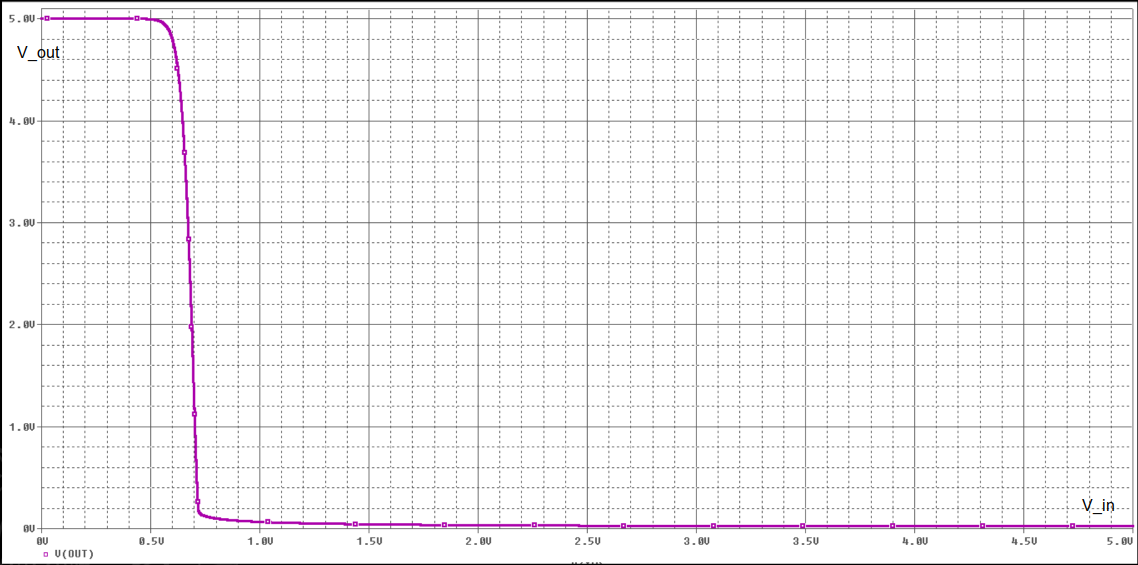
\includegraphics[width=\textwidth]{assets/imgs/grafico_not_rtl.png}
\caption{Grafico della porta NOT RTL.}
\label{fig:subfig1} \end{subfigure}
\hspace*{\fill}
\begin{subfigure}{.45\textwidth}
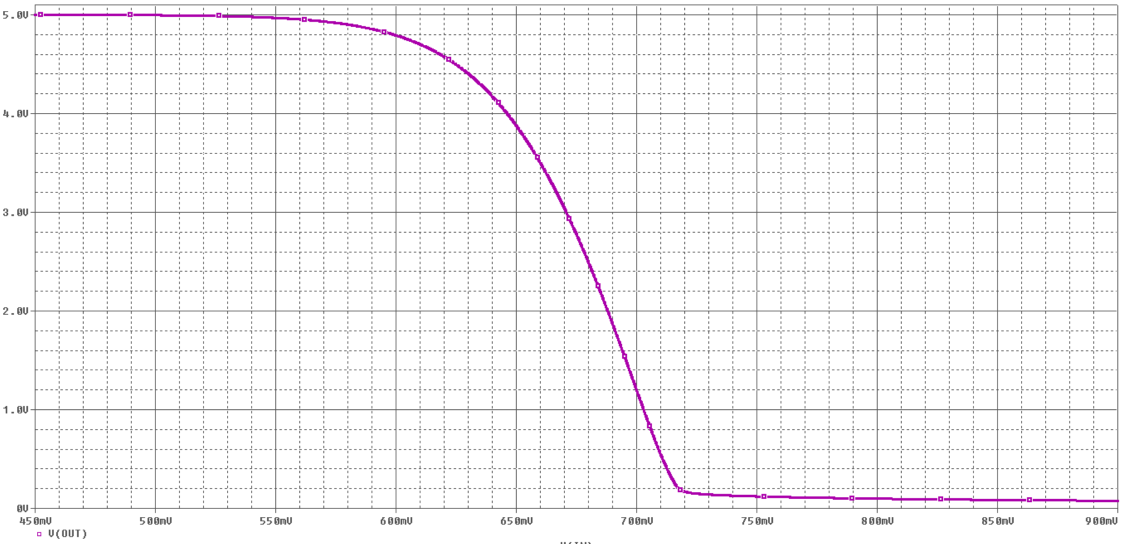
\includegraphics[width=\textwidth]{assets/imgs/ingrandimento_grafico_not.png}
\caption{Ingrandimento tra $0,5 V$ e  $1V$} \label{fig:subfig2}
\end{subfigure}
\caption{Grafici sulla funzione di trasferimento} \label{fig:grafici rtl_not}
\end{figure}

Bisogna però stabilire se la famiglia logica sia ``buona'' o meno
tramite i valori di \(V_{iH}\) e \(V_{iL}\). Per far ciò utilizziamo un
simulatore di circuiti elettrici, all'interno del quale sono inseriti
sia i parametri che la descrizione del circuito stesso e farne un
grafico. Il primo rappresenta della funzione di trasferimento della
porta NOT, ottenuto. Il grafico si dice \textbf{statico}, in quanto non
è presente la variabile temporale. Sull'asse delle ascisse è presente la
tensione in ingresso, mentre sulle ordinate è presente la tensione di
uscita. \newline Sappiamo dal grafico che esso rappresenta la porta NOT
in quanto se l'ingresso è basso, l'uscita è alta e viceversa (sopra
certi valori). In una zona tra gli \(0,5V\) e \(0,7V\) si ha la
commutazione.\newline Il secondo grafico è un ingrandimento del primo,
viene evidenziata la zona della commutazione: a \(600mV\) viene definito
il punto in cui la giunzione base emettitore si accende. Ciò significa
che si sta accendendo anche il transistor (sta iniziando a
polarizzarsi), quindi scorre corrente in base e di conseguenza anche
sulla resistenza di collettore, e la tensione (del collettore) in uscita
diminuisce (drasticamente). Quindi dai \(700mV\) il transistor è in
saturazione, ma vogliamo dare alla tensione in ingresso minimo
\(750mV\). Abbiamo quindi trovato \(V_{iH}\) e \(V_{iL}\). La tensione
in uscita \(V_{oL}\) è semplice trovarla sugli
\(\approx 0,2V = V_{CE-sat}\), mentre \(V_{oH}\) è più particolare,
perché senza nessun carico è pari a \(5V\). \newline Osserviamo inoltre
che il noise margin è particolarmente basso, dovuto alla differenza tra
i valori delle tensioni associati agli stati logici bassi.

\subsubsection{Calcolo del Fan-out}\label{calcolo-del-fan-out}

Sappiamo che all'uscita di un transistor si possono collegare più
ingressi: potenzialmente un numero \(n\)

\begin{figure}[H]
    \centering
    \resizebox{0.5\textwidth}{!}{\documentclass[tikz,border=10pt]{standalone}
\usepackage{circuitikz}

\begin{document}
\begin{circuitikz}
	% Paths, nodes and wires:
	\draw (2, 10) to[american resistor] (2, 7);
	\draw node[npn] at (2, 6.23) {};
	\draw[-latex] (2, 7) -- (5, 7);
	\node[shape=rectangle, draw, line width=1pt, inner sep=0, minimum width=-0.035cm, minimum height=-0.035cm] at (4.75, 7.5){};
	\node[shape=rectangle, inner sep=0, minimum width=0.634cm, minimum height=0.134cm](Rect1) at (4.875, 7.375){} node[anchor=center] at (Rect1.center){$I_{out}$};
	\draw node[circ] (N1) at (3.5, 7) {} node[anchor=north] at (N1.south){$V_{out}$};
	\draw (5, 7) -- (6, 7);
	\draw (6, 10) -| (6, 7) -| (6, 10);
	\draw (6, 10) to[american resistor] (9, 10);
	\draw (6, 8) to[american resistor] (9, 8);
	\draw (6, 6.25) to[american resistor] (9, 6.25);
	\draw (6, 7) -- (6, 6.25);
	\draw node[ground] at (2, 5.46) {};
	\draw[dash pattern={on 1.6pt off 1.6pt}] (6, 6.25) -| (6, 4);
	\draw node[npn, xscale=0.8, yscale=0.8] (N2) at (9.672, 10) {} node[anchor=west] at (N2.east){$1$};
	\draw node[npn, xscale=0.8, yscale=0.8] (N3) at (9.672, 8) {} node[anchor=west] at (N3.text){$2$};
	\draw node[npn, xscale=0.8, yscale=0.8] (N4) at (9.672, 6.25) {} node[anchor=west] at (N4.text){$3$};
	\draw (6, 4) to[american resistor] (9, 4);
	\draw node[npn, xscale=0.8, yscale=0.8] (N5) at (9.672, 4) {} node[anchor=west] at (N5.text){$n$};
\end{circuitikz}
\end{document}
}
    \caption{Uscita per calcolo fanout: da un transistor si collegano n ingressi, composti da una resistenza ed una giunzione base-emettitore}
\end{figure}

\begin{itemize}
\tightlist
\item
  Se vogliamo un valore \emph{alto} su \(V_{OUT}\), questo deve essere
  pari (condizione limite) alla tensione \(V_{iH}=0,75V\). Inoltre:
  \begin{align*}
  \left. \begin{array}{l} 
  V_{RC}=5-0,75 \: V=4,25 V \\
  R_{C}=640\Omega
  \end{array} \right\} 
  \Longrightarrow 
  I_{out}=\frac{4,25V}{640\Omega}=6,6\:mA \\
  I_{iH}@0,75V=150\:\mu A \Longrightarrow \frac{6,6\:mA}{150\:\mu A}=44 \text{ porte logiche.}
  \end{align*} che rispetto al valore espresso sul datasheet, ovvero 33,
  è maggiore. Tuttavia si utilizza quest'ultimo valore al fine di
  lasciare un po' di margine al circuito (considerando \(I_H=200\mu A\))
\item
  Per avere un valore \emph{basso} su \(V_{out}\): se l'uscita bassa con
  corrente \(I_{iL}\simeq 0\), teoricamente non vi è un limite sul
  numero di porte logiche.
\end{itemize}

\subsubsection{Calcolo della potenza
statica}\label{calcolo-della-potenza-statica}

\begin{itemize}
\tightlist
\item
  Potenza dissipata se l'uscita è \emph{bassa}: \begin{align*}
  \left. \begin{array}{l} 
  V_{RC}=5-0,2 \: V=4,8 V \\
  i_{C}=\frac{4,8\:V}{640\Omega}=7,5\:mA
  \end{array} \right\} 
  \Longrightarrow 
  P_{L}=5\:V\cdot 7,5\:mA=37,5\:mW
  \end{align*}
\item
  Potenza dissipata se l'uscita è \emph{alta}: \begin{align*}
  V_{out}=5\:V\Longrightarrow V_{RC}=0\Longrightarrow I_{C}=0\Longrightarrow P_{H}=0\:mW
  \end{align*} Si considera carico \textbf{\emph{nullo}}: la porta non è
  collegata ad altre porte.
\end{itemize}

\subsubsection{Tempi di propagazione:}\label{tempi-di-propagazione}

\begin{itemize}
\tightlist
\item
  \(t_{p_{HL}}\) è pari al tempo necessario a polarizzare la giunzione
  p-n: pochi nS;
\item
  \(t_{p_{LH}}\) è pari al tempo necessario a rimuovere i portatori
  minoritari dalla base, ovvero il tempo necessario a spegnere la
  giunzione p-n: pochi nS;
\end{itemize}

L'ultimo parametro dinamico è il \emph{Delay-power product}:
\(DP=5\:ns\cdot 18\:mW=90\:pJ\)

\begin{redbox}{Osservazione}
Se incrementiamo la resistenza di base (aumentando da $450\Omega$) \emph{diminuisce la potenza ma aumenta il tempo}.\newline
Tuttavia i valori scelti per le resistenza ottimizzano le prestazioni di tutta la famiglia logica RTL.
\end{redbox}
\begin{orangebox}{Problemi della famiglia RTL}
Uno dei problemi principali della famiglia logia RTL è il fatto che lo stadio d'ingresso formato da una resistenza e dalla giunzione base-emettitore assorbe molta corrente in un verso e non ne assorbe nell'altro.
\end{orangebox}

\section{TTL
(transistor-transistor-logic)}\label{ttl-transistor-transistor-logic}

È una famiglia logica successiva alla famiglia RTL, ed è più
\emph{evoluta}: le porte logiche in questo caso sono realizzati
utilizzando una \textbf{\emph{coppia di transistori}}:

\begin{figure}[H]
    \centering
    \resizebox{0.5\textwidth}{!}{\begin{tikzpicture}
	% Paths, nodes and wires:
	\draw node[pnp, rotate=-90, xscale=1.28, yscale=1.28] (N1) at (2.014, 7) {} node[anchor=north] at (N1.text){$Q1$};
	\draw (2, 11) to[american resistor, l_={$\text{RPU}$}, label distance=0.02cm] (2.014, 8.075);
	\draw node[npn, xscale=1.22, yscale=1.22] (N2) at (6.025, 7) {} node[anchor=south east] at ([xshift=0.62cm, yshift=-0.62cm]N2.north west){$Q2$};
	\draw (3, 7) -- (5, 7);
	\draw (6, 11) to[american resistor, l_={$\text{R}_{\text{C}}$}, label distance=0.02cm] (6.025, 7.939);
	\draw (6, 8) -- (7, 8);
	\draw (6.025, 6.061) |- (6, 5);
	\draw node[ground, xscale=1.2, yscale=1.2] (N3) at (6.025, 5) {} node[anchor=north west] at ([xshift=-0.1cm, yshift=0.1cm]N3.south east){$0$};
	\draw node[ocirc] (N4) at (7, 8) {} node[anchor=west] at (N4.east){$OUT$};
	\draw node[ocirc] (N5) at (1.029, 7) {} node[anchor=east] at (N5.west){$IN$};
	\draw node[ocirc] (N6) at (6, 11) {} node[anchor=south] at (N6.north){$5V$};
	\draw node[ocirc] (N7) at (2, 11) {} node[anchor=south] at (N7.north){$5V$};
	\node[shape=rectangle, inner sep=0, minimum width=0.715cm, minimum height=0.465cm](Rect1) at (2.625, 9.5){} node[anchor=center] at (Rect1.center){$4k\Omega$};
	\node[shape=rectangle, inner sep=0, minimum width=0.715cm, minimum height=0.465cm](Rect2) at (6.75, 9.5){} node[anchor=center] at (Rect2.center){$1,6k\Omega$};
	\node[shape=rectangle, inner sep=0, minimum width=0.465cm, minimum height=0.215cm](Rect3) at (2.25, 7.75){} node[anchor=center] at (Rect3.center){$\text{B}$};
	\node[shape=rectangle, inner sep=0, minimum width=0.215cm, minimum height=0.215cm](Rect4) at (1.375, 6.75){} node[anchor=center] at (Rect4.center){$\text{E}$};
	\node[shape=rectangle, inner sep=0, minimum width=0.215cm, minimum height=0.215cm](Rect5) at (3, 6.75){} node[anchor=center] at (Rect5.center){$\text{C}$};
	\node[shape=rectangle, inner sep=0, minimum width=0.465cm, minimum height=0.061cm](Rect6) at (5, 6.75){} node[anchor=center] at (Rect6.center){$\text{B}$};
	\node[shape=rectangle, inner sep=0, minimum width=0.465cm, minimum height=0.061cm](Rect7) at (6.25, 6.298){} node[anchor=center] at (Rect7.center){$\text{E}$};
	\node[shape=rectangle, inner sep=0, minimum width=0.215cm, minimum height=0.215cm](Rect8) at (5.75, 7.75){} node[anchor=center] at (Rect8.center){$\text{C}$};
\end{tikzpicture}
}
    \caption{Porta NOT "semplice" in TTL.}
\end{figure}

\subsubsection{\texorpdfstring{Porta \textbf{Basic
NOT}:}{Porta Basic NOT:}}\label{porta-basic-not}

Durante le transizioni dallo stato basso ad alto i portatori minoritari
presenti in Q2 vengono rimossi dal transistor Q1; se l'ingresso della
porta logica è \textbf{basso/spento} (ad esempio la tensione in ingresso
\(V_{in}=0,2V\)) la giunzione base-emettitore Q1 sarà accesa (grazie
alla resistenza RPU, resistenza di pull-up, che porta i \(5V\) in
ingresso) e quindi scorre della corrente in base nel transistor Q1. La
giunzione può essere in regione attiva diretta oppure in saturazione:
tuttavia per essere in regione attiva dovrebbe esserci un ingresso di
corrente nel collettore di Q1, ma in condizioni stazionarie ciò non
accade perché per la disposizione del transistor Q2 non scorre corrente
verso il collettore, quindi Q1 si trova in saturazione. Di conseguenza
la tensione sulla base del transistor Q2 (= tensione di collettore di
Q1) sarà pari a \(V_{in}+0,2V=0,2V\), che è troppo \emph{bassa} per
accendere il transistor Q2: per questo motivo tutta la corrente andrà in
uscita.

\begin{greenbox}{Memo}
La giunzione base-collettore è anch'essa assimilabile ad un diodo, per cui ha il suo massimo potenziale a $\approx 0,7V$
\end{greenbox}

Quando l'ingresso è a 5V, il transistor entra in regione attiva inversa,
caratterizzata da un guadagno molto basso. Di conseguenza, nel
collettore fluisce quasi esclusivamente la corrente di base. Con questa
famiglia logica, il problema dell'assorbimento di corrente si manifesta
principalmente quando il transistor viene acceso. Tuttavia, tale
assorbimento è inferiore poiché il transistor opera già in saturazione.
Inoltre, questo comportamento rende la porta più prevedibile nel
funzionamento.

A causa delle oscillazioni dei valori la tensione in \(V_{B}=0-0,75V\),
mentre la tensione sul collettore \(V_{C}=0-1,5V\). Se invece abbiamo un
ingresso alto (tensione in ingresso \(V_{in}=5V\)), Q1 si troverà in
regione attiva inversa, con gain quasi nullo.

\begin{figure}[H]
    \centering
    \resizebox{0.5\textwidth}{!}{\begin{tikzpicture}
	% Paths, nodes and wires:
	\draw (2, 11) to[american resistor, l_={$\text{RPU}$}, label distance=0.02cm] (2.014, 8.075);
	\draw node[npn, xscale=1.22, yscale=1.22] (N1) at (6.025, 7) {} node[anchor=south east] at ([xshift=0.62cm, yshift=-0.62cm]N1.north west){$Q2$};
	\draw (3, 7) -- (5, 7);
	\draw (6, 11) to[american resistor, l_={$\text{R}_{\text{C}}$}, label distance=0.02cm] (6.025, 7.939);
	\draw (6, 8) -- (7, 8);
	\draw (6.025, 6.061) |- (6, 5);
	\draw node[ground, xscale=1.2, yscale=1.2] (N2) at (6.025, 5) {} node[anchor=north west] at ([xshift=-0.1cm, yshift=0.1cm]N2.south east){$0$};
	\draw node[ocirc] (N3) at (7, 8) {} node[anchor=west] at (N3.east){$OUT$};
	\draw node[ocirc] (N4) at (6, 11) {} node[anchor=south] at (N4.north){$5V$};
	\draw node[ocirc] (N5) at (2, 11) {} node[anchor=south] at (N5.north){$5V$};
	\node[shape=rectangle, inner sep=0, minimum width=0.715cm, minimum height=0.465cm](Rect1) at (2.625, 9.5){} node[anchor=center] at (Rect1.center){$4k\Omega$};
	\node[shape=rectangle, inner sep=0, minimum width=0.715cm, minimum height=0.465cm](Rect2) at (6.75, 9.5){} node[anchor=center] at (Rect2.center){$1,6k\Omega$};
	\draw (2.014, 8.075) to[empty diode] (2.014, 7.075);
	\draw (2.014, 7.075) |- (3, 7);
	\draw[-stealth] (1.5, 7.5) -| (1.5, 6.75) -- (2.5, 6.75);
	\node[shape=rectangle, inner sep=0, minimum width=0.965cm, minimum height=0.465cm](Rect3) at (1.75, 6.25){} node[anchor=center] at (Rect3.center){$i_{Q1}$};
\end{tikzpicture}}
    \caption{Porta NOT "semplice" con Q1 diodo.}
\end{figure}

Q1 diventa assimilabile ad un diodo, mandando tutta la corrente verso la
base del transistor Q2: in questo modo essa va in saturazione, ottenendo
un'uscita bassa (come nella porta NOT nella logica RTL). È da notare che
attraverso Q1 la corrente di scarica di Q2 viene aumentata
considerevolmente e di conseguenza si potrà spegnere velocemente: la
transizione dell'uscita da basso ad altro è molto veloce.

\begin{redbox}{In sintesi:}
\begin{itemize}
\item Transizioni dallo stato basso ad alto \emph{veloci}, dato che il transistor Q1 aiuta a smaltire le cariche minoritarie immagazzinate da Q2;
\item L'uscita deve comunque essere tirata verso l'alto\footnote{Aumentare la tensione o portare un segnale verso un valore più alto.} da $R_C$
\item L'ingresso assorbe corrente sole se basso, ed è in funzione di $RPU$
\end{itemize}
\end{redbox}

\subsubsection{Enhanced NOT}\label{enhanced-not}

Viene disegnato un nuovo circuito per migliorare le prestazioni: in
particolare l'uscita, se positiva, non è governata dal transistor, ma
dalla resistenza di collettore.\newline Consideriamo quindi un circuito
migliorato:

\begin{figure}[H]
    \centering
    \resizebox{0.6\textwidth}{!}{\begin{tikzpicture}
	% Paths, nodes and wires:
	\draw node[pnp, rotate=-90, xscale=1.28, yscale=1.28] (N1) at (2.014, 7) {} node[anchor=north] at (N1.text){$Q1$};
	\draw (2, 11) to[american resistor, l_={$\text{RPU}$}, label distance=0.02cm] (2.014, 8.075);
	\draw node[npn, xscale=1.22, yscale=1.22] (N2) at (9.525, 5) {} node[anchor=west] at ([xshift=-0.02cm]N2.east){$Q2$};
	\draw (3, 7) -- (5, 7);
	\draw (6, 11) to[american resistor, l_={$\text{RPU}'$}, label distance=0.02cm] (6, 7.939);
	\draw (9.525, 5.892) -- (10.525, 5.892);
	\draw (9.525, 4.061) |- (9.5, 3);
	\draw node[ground, xscale=1.2, yscale=1.2] (N3) at (9.525, 3) {} node[anchor=north west] at ([xshift=-0.1cm, yshift=0.1cm]N3.south east){$0$};
	\draw node[ocirc] (N4) at (10.525, 5.892) {} node[anchor=west] at (N4.east){$OUT$};
	\draw node[ocirc] (N5) at (1.029, 7) {} node[anchor=east] at (N5.west){$IN$};
	\draw node[ocirc] (N6) at (6, 11) {} node[anchor=south] at (N6.north){$5V$};
	\draw node[ocirc] (N7) at (2, 11) {} node[anchor=south] at (N7.north){$5V$};
	\node[shape=rectangle, inner sep=0, minimum width=0.715cm, minimum height=0.465cm](Rect1) at (2.625, 9.5){} node[anchor=center] at (Rect1.center){$4k\Omega$};
	\node[shape=rectangle, inner sep=0, minimum width=0.715cm, minimum height=0.465cm](Rect2) at (6.75, 9.5){} node[anchor=center] at (Rect2.center){$1,6k\Omega$};
	\draw node[npn, xscale=1.22, yscale=1.22] (N8) at (6, 7) {} node[anchor=south east] at ([xshift=0.62cm, yshift=-0.62cm]N8.north west){$Q3$};
	\draw (6, 5) to[american resistor, l_={$\text{RPD}$}, label distance=0.02cm] (6, 3);
	\draw node[npn, xscale=1.22, yscale=1.22] (N9) at (9.525, 8) {} node[anchor=west] at ([xshift=-0.02cm]N9.east){$Q4$};
	\draw (9.525, 7.061) to[empty diode, l={$\text{D1}$}, label distance=0.02cm,/tikz/circuitikz/bipoles/length=0.980cm] (9.525, 5.892);
	\draw (6, 6.061) -- (6, 5) -- (8.5, 5);
	\draw (9.5, 11) to[american resistor, l_={$\text{R}_{\text{C}}$}, label distance=0.02cm] (9.525, 8.939);
	\draw (8.5, 8) -- (6, 8);
	\node[shape=rectangle, inner sep=0, minimum width=0.715cm, minimum height=0.465cm](Rect3) at (10.25, 10){} node[anchor=center] at (Rect3.center){$130\Omega$};
	\draw node[ocirc] (N10) at (9.5, 11) {} node[anchor=south] at (N10.north){$5V$};
	\draw node[ground, xscale=1.2, yscale=1.2] (N11) at (6, 3) {} node[anchor=north west] at ([xshift=-0.1cm, yshift=0.1cm]N11.south east){$0$};
	\draw[draw={rgb,255:red,97;green,53;blue,131}, line width=3pt] (5, 2.5) -| (5, 2) -- (7, 2) -| (7, 2.5);
	\draw[draw={rgb,255:red,26;green,95;blue,180}, line width=3pt] (8.5, 2.5) -| (8.5, 2) -- (10.5, 2) -| (10.5, 2.5);
	\node[shape=rectangle, inner sep=0, minimum width=1.965cm, minimum height=0.715cm](Rect4) at (6, 1.375){} node[anchor=center] at (Rect4.center){$\text{Phase Splitter}$};
	\node[shape=rectangle, line width=0pt, inner sep=0, minimum width=2cm, minimum height=0.75cm](Rect5) at (9.5, 1.375){} node[anchor=center] at (Rect5.center){$\text{Totem Pole}$};
\end{tikzpicture}
}
    \caption{Enhanced NOT.}
\end{figure}

Il sottocircuito \textbf{\emph{phase splitter}} si occupa di generare
due segnali \emph{complementari}: se il collettore è alto l'emettitore è
basso e viceversa.

Il funzionamento di questo circuito è un'estensione della porta logica
NOT base: il transistor Q3 pilota l'uscita in modo tale che soltanto uno
dei due transistor Q2 e Q4 sia acceso!

\begin{bluebox}{Caratteristiche della porta logica Enhanced Not}
\begin{itemize}
\item Q4 "tira su" la (tensione di ) uscita \emph{rapidamente}. Tuttavia, come visto in precedenza un transistor si spegne molto più lentamente di quanto si accenda: esiste quindi la possibilità che il transistor Q4 si accenda \emph{\textbf{prima}} che si spenga Q2 (questo viene detto fenomeno di \emph{cross-conduction}). Per evitarlo si rallenta l'accensione di Q4 ponendo una resistenza di collettore $R_C$.
\item Come spiegato nel punto precedente, il transistor Q2 si spegne più lentamente (commutazione tra L e H), perché non c'è più Q1 ad assorbire. Per limitare il problema di utilizza una resistenza di \emph{pull-down} RPD.
\end{itemize}
\end{bluebox}

Analizziamo il grafico di funzionamento della porta NOT, dove sull'asse
delle ascisse abbiamo la tensione in ingresso, mentre sull'asse delle
ordinate abbiamo la tensione in uscita:

\begin{figure}
\centering
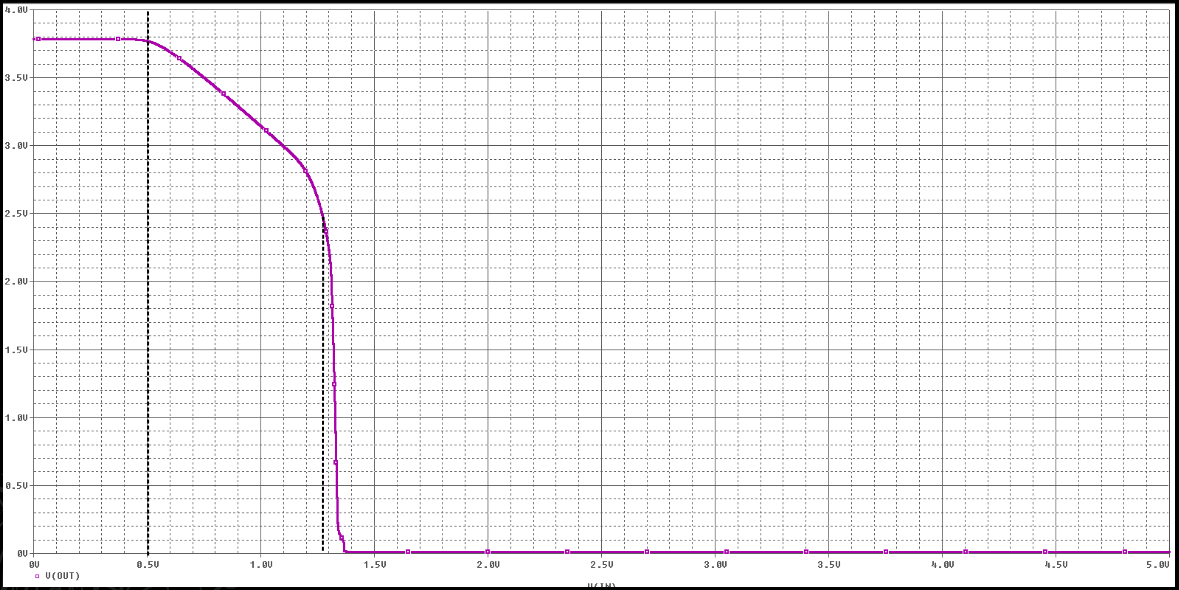
\includegraphics[width=0.6\linewidth,height=\textheight,keepaspectratio]{assets/imgs/enhanced_not.png}
\caption{Grafico porta enhanced NOT.}
\end{figure}

Il porta si trova nella \textbf{regione lineare} tra gli \(0,6\) e gli
\(1,2V\): Q3 si sta accendendo, sulla seconda resistenza di pull-up RPU'
cade un potenziale proporzionale alla corrente che Q3 inizia a far
scorrere. Tale caduta si riflette sul transistor Q4. Dopodiché subito
dopo \(1,2V\) si ha una ripida caduta di tensione causata
dall'accensione del transistor Q2.\newline Si può osservare come in
uscita non otteniamo mai una tensione pari a \(5V\): questo a causa
delle cadute di potenziale sul transistor Q4 e sul diodo D1.\newline
Tuttavia questo circuito non è ancora il migliore possibile, in quanto
vorremmo delle funzioni che siano più ``ripide''. Per ovviare a ciò si
aggiunge un altro sottocircuito al \emph{phase splitter} e al
\emph{totem pole}: il sottocircuito \textbf{\emph{active pull-down}}.

\subsubsection{Standard NOT}\label{standard-not}

\begin{figure}[H]
    \centering
    \resizebox{0.8\textwidth}{!}{\begin{tikzpicture}
	% Paths, nodes and wires:
	\draw node[pnp, rotate=-90, xscale=1.28, yscale=1.28] (N1) at (2.014, 7) {} node[anchor=north] at (N1.text){$Q1$};
	\draw (2, 11) to[american resistor, l_={$\text{RPU}$}, label distance=0.02cm] (2.014, 8.075);
	\draw node[npn, xscale=1.22, yscale=1.22] (N2) at (10.9, 5) {} node[anchor=west] at ([xshift=-0.02cm]N2.east){$Q2$};
	\draw (3, 7) -- (5, 7);
	\draw (6, 11) to[american resistor, l_={$\text{RPU}'$}, label distance=0.02cm] (6, 7.939);
	\draw (10.9, 5.892) -- (11.9, 5.892);
	\draw (10.9, 4.061) |- (10.875, 3);
	\draw node[ground, xscale=1.2, yscale=1.2] (N3) at (10.9, 3) {} node[anchor=north west] at ([xshift=-0.1cm, yshift=0.1cm]N3.south east){$0$};
	\draw node[ocirc] (N4) at (11.9, 5.892) {} node[anchor=west] at (N4.east){$OUT$};
	\draw node[ocirc] (N5) at (1.029, 7) {} node[anchor=east] at (N5.west){$IN$};
	\draw node[ocirc] (N6) at (6, 11) {} node[anchor=south] at (N6.north){$5V$};
	\draw node[ocirc] (N7) at (2, 11) {} node[anchor=south] at (N7.north){$5V$};
	\node[shape=rectangle, inner sep=0, minimum width=0.715cm, minimum height=0.465cm](Rect1) at (2.625, 9.5){} node[anchor=center] at (Rect1.center){$4k\Omega$};
	\node[shape=rectangle, inner sep=0, minimum width=0.715cm, minimum height=0.465cm](Rect2) at (6.75, 9.5){} node[anchor=center] at (Rect2.center){$1,6k\Omega$};
	\draw node[npn, xscale=1.22, yscale=1.22] (N8) at (6, 7) {} node[anchor=south east] at ([xshift=0.62cm, yshift=-0.62cm]N8.north west){$Q3$};
	\draw (6, 5) to[american resistor, l_={$\text{RPU2}$}, label distance=0.02cm] (6, 3);
	\draw node[npn, xscale=1.22, yscale=1.22] (N9) at (10.9, 8) {} node[anchor=west] at ([xshift=-0.02cm]N9.east){$Q4$};
	\draw (10.9, 7.061) to[empty diode, l={$\text{D1}$}, label distance=0.02cm,/tikz/circuitikz/bipoles/length=0.980cm] (10.9, 5.892);
	\draw (6, 6) |- (7.375, 5) -- (9.875, 5);
	\draw (10.875, 11) to[american resistor, l_={$\text{R}_{\text{C}}$}, label distance=0.02cm] (10.9, 8.939);
	\draw (9.875, 8) -- (6, 8);
	\node[shape=rectangle, inner sep=0, minimum width=0.715cm, minimum height=0.465cm](Rect3) at (11.625, 10){} node[anchor=center] at (Rect3.center){$130\Omega$};
	\draw node[ocirc] (N10) at (10.875, 11) {} node[anchor=south] at (N10.north){$5V$};
	\node[shape=rectangle, draw, line width=0pt, inner sep=0, minimum width=2cm, minimum height=0.75cm](Rect4) at (14.25, 6.75){} node[anchor=center] at (Rect4.center){$\text{Totem Pole}$};
	\node[shape=rectangle, inner sep=0, minimum width=0.715cm, minimum height=1.215cm](Rect5) at (5.375, 3.625){} node[anchor=center] at (Rect5.center){$500\Omega$};
	\draw (8.25, 5) to[american resistor, l_={$\text{RPD}$}, label distance=0.02cm] (8.25, 3);
	\draw node[ground, xscale=1.2, yscale=1.2] (N11) at (8.25, 1.48) {} node[anchor=north west] at ([xshift=-0.1cm, yshift=0.1cm]N11.south east){$0$};
	\node[shape=rectangle, inner sep=0, minimum width=0.715cm, minimum height=0.465cm](Rect6) at (8.875, 4){} node[anchor=center] at (Rect6.center){$250\Omega$};
	\draw node[npn] (N12) at (8.25, 2.25) {} node[anchor=south east] at ([xshift=0.51cm, yshift=-0.51cm]N12.north west){$Q5$};
	\draw (6, 3) -| (6, 2.25) -- (7.41, 2.25);
	\draw[draw={rgb,255:red,97;green,53;blue,131}, line width=1.2pt] (4.75, 5.25) -- (4.75, 1.25) -- (9.25, 1.25) -| (9.5, 5.25) -- (4.75, 5.25);
	\node[shape=rectangle, inner sep=0, minimum width=1.965cm, minimum height=0.715cm](Rect7) at (6.25, 0.875){} node[anchor=center] at (Rect7.center){$\text{Active Pull Down}$};
	\draw[draw={rgb,255:red,224;green,27;blue,36}, line width=1.1pt] (10, 11.5) -| (10, 2.75) -| (13, 3) |- (12.25, 11.75) |- (10, 11.75) -| (10, 11.5);
\end{tikzpicture}}
    \caption{Standard NOT.}
\end{figure}

Il sottocircuito active pull-down (APD) è \emph{attivo} perché
sostituisce la resistenza di pull down, che era passiva. Infatti una
tensione nel punto P accende il transistor Q5, che fa da ``pozzo''. Il
fatto di essere un ``componente attivo'' implica inoltre altre due cose:

\begin{enumerate}
\def\labelenumi{\arabic{enumi})}
\tightlist
\item
  È più rapido a spegnere il transistor Q2 al momento opportuno;
\item
  Sincronizza, al momento dell'accensione del circuito, l'accensione dei
  transistor Q2 e Q3 e lo spegnimento di Q4: infatti il transistor Q5
  viene detto \emph{sincronizzatore}. Esso si accende insieme a Q2 e
  sottrae corrente alla base di Q4.
\end{enumerate}

Tutto ciò rende il grafico \emph{più ripido}:

\begin{figure}
\centering
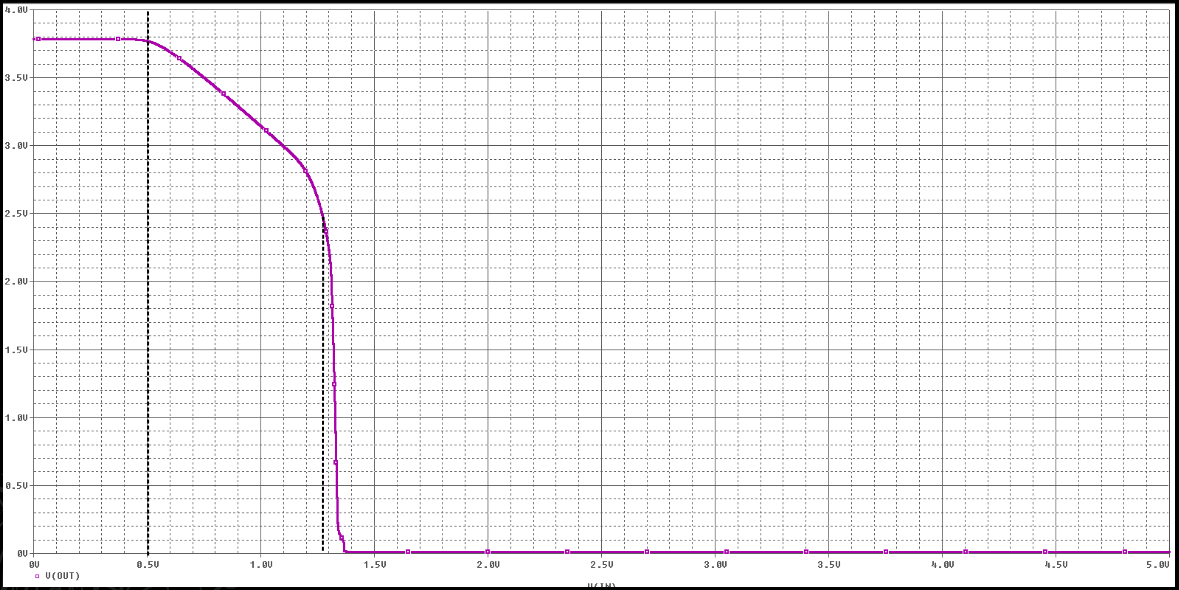
\includegraphics[width=0.6\linewidth,height=\textheight,keepaspectratio]{assets/imgs/standard_not.png}
\caption{Grafico di trasferimento della porta Standard NOT in TTL.}
\end{figure}

L'aggiunta di un nuovo transistor si è rivelata una scelta eccellente,
poiché questa porta non solo è più veloce rispetto alla versione
enhanced, ma consuma anche meno energia. Questo miglioramento è dovuto
al fatto che, nell'intervallo di tempo tra il momento in cui l'input
passa a 0 e l'output sale a 1 (circa 10 ns), il circuito assorbe
corrente. Grazie al transistor aggiunto, questa finestra temporale è
stata quasi dimezzata, riducendo significativamente il consumo di
corrente. La resistenza RC da \(130\Omega\) serve per ridurre la
corrente che passa quando, durante la commutazione, sia Q2 che Q4 sono
chiusi e quindi la corrente va verso la massa.

\subsubsection{Parametri TTL}\label{parametri-ttl}

\begin{itemize}
\tightlist
\item
  \(V_{iH}=1,35V, \qquad V_{iL}=1,1V\)
\item
  \(I_{iH}\sim 1,5\mu A, \qquad I_{iL}=1\mu A\)
\item
  \(V_{oH}=3,75V, \qquad V_{oL}=0,2V\)
\item
  \(NM_H = 2.4V, NM_L : 0.9V \to NM = 0.9V\)
\item
  \begin{flalign*}
  &\begin{aligned}
  &\left. \begin{array}{l} 
  P_{L}=5V(\underbrace{0,7mA}_{R_{PU}}+\underbrace{2,5mA}_{R_{PU}'})=16mW \\
  P_{L}=5V(\underbrace{1mA}_{R_{PU}})=5mW
  \end{array} \right\} 
  \Longrightarrow 
  P=11,5mW
  \end{aligned}&&
  \end{flalign*}
\item
  \(t_{p_{HL}} \sim t_{p_{HL}} \sim 5 nS, \quad PD=5nS\cdot 11,5 mW=57,5 pJ\)
\end{itemize}

\subsubsection{Ulteriori porte logiche in
TTL}\label{ulteriori-porte-logiche-in-ttl}

Per realizzare tutte le funzioni è tuttavia necessario implementare
almeno la porta NAND oppure la porta NOR. Tra le due la più semplice è
la prima, che è uguale alla standard NOT, tranne per la presenza di un
transistor \textbf{multi-emettitore}.

\begin{figure}[H]
    \centering
    \resizebox{0.5\textwidth}{!}{\begin{tikzpicture}
	% Paths, nodes and wires:
	\draw (2, 11) to[american resistor, l_={$\text{RPU}$}, label distance=0.02cm] (2, 7.84);
	\draw node[npn, xscale=1.22, yscale=1.22] (N1) at (10.9, 5) {} node[anchor=west] at ([xshift=-0.02cm]N1.east){$Q2$};
	\draw (2.77, 7) |- (5, 7);
	\draw (6, 11) to[american resistor, l_={$\text{RPU}'$}, label distance=0.02cm] (6, 7.939);
	\draw (10.9, 5.892) -- (11.9, 5.892);
	\draw (10.9, 4.061) |- (10.875, 3);
	\draw node[ground, xscale=1.2, yscale=1.2] (N2) at (10.9, 3) {} node[anchor=north west] at ([xshift=-0.1cm, yshift=0.1cm]N2.south east){$0$};
	\draw node[ocirc] (N3) at (11.9, 5.892) {} node[anchor=west] at (N3.east){$\overline{A+B}$};
	\draw node[ocirc] (N4) at (6, 11) {} node[anchor=south] at (N4.north){$5V$};
	\draw node[ocirc] (N5) at (2, 11) {} node[anchor=south] at (N5.north){$5V$};
	\node[shape=rectangle, inner sep=0, minimum width=0.715cm, minimum height=0.465cm](Rect1) at (2.625, 9.5){} node[anchor=center] at (Rect1.center){$4k\Omega$};
	\node[shape=rectangle, inner sep=0, minimum width=0.715cm, minimum height=0.465cm](Rect2) at (6.75, 9.5){} node[anchor=center] at (Rect2.center){$1,6k\Omega$};
	\draw node[npn, xscale=1.22, yscale=1.22] (N6) at (6, 7) {} node[anchor=south east] at ([xshift=0.62cm, yshift=-0.62cm]N6.north west){$Q3$};
	\draw (6, 5) to[american resistor, l_={$\text{RPU2}$}, label distance=0.02cm] (6, 3);
	\draw node[npn, xscale=1.22, yscale=1.22] (N7) at (10.9, 8) {} node[anchor=west] at ([xshift=-0.02cm]N7.east){$Q4$};
	\draw (10.9, 7.061) to[empty diode, l={$\text{D1}$}, label distance=0.02cm,/tikz/circuitikz/bipoles/length=0.980cm] (10.9, 5.892);
	\draw (6, 6) |- (7.375, 5) -- (9.875, 5);
	\draw (10.875, 11) to[american resistor, l_={$\text{R}_{\text{C}}$}, label distance=0.02cm] (10.9, 8.939);
	\draw (9.875, 8) -- (6, 8);
	\node[shape=rectangle, inner sep=0, minimum width=0.715cm, minimum height=0.465cm](Rect3) at (11.625, 10){} node[anchor=center] at (Rect3.center){$130\Omega$};
	\draw node[ocirc] (N8) at (10.875, 11) {} node[anchor=south] at (N8.north){$5V$};
	\node[shape=rectangle, inner sep=0, minimum width=0.715cm, minimum height=1.215cm](Rect4) at (5.375, 3.625){} node[anchor=center] at (Rect4.center){$500\Omega$};
	\draw (8.25, 5) to[american resistor, l_={$\text{RPD}$}, label distance=0.02cm] (8.25, 3);
	\draw node[ground, xscale=1.2, yscale=1.2] (N9) at (8.25, 1.48) {} node[anchor=north west] at ([xshift=-0.1cm, yshift=0.1cm]N9.south east){$0$};
	\node[shape=rectangle, inner sep=0, minimum width=0.715cm, minimum height=0.465cm](Rect5) at (8.875, 4){} node[anchor=center] at (Rect5.center){$250\Omega$};
	\draw node[npn] (N10) at (8.25, 2.25) {} node[anchor=south east] at ([xshift=0.51cm, yshift=-0.51cm]N10.north west){$Q5$};
	\draw (6, 3) -| (6, 2.25) -- (7.41, 2.25);
	\draw node[npn, rotate=-90] at (2, 7) {};
	\draw node[npn, rotate=-90] at (2, 5.5) {};
	\node[shape=rectangle, inner sep=0, minimum width=0.465cm, minimum height=0.465cm](Rect6) at (0.98, 7){} node[anchor=center] at (Rect6.center){$\text{A}$};
	\draw (2, 7.84) -| (2, 6.34);
	\node[shape=rectangle, inner sep=0, minimum width=0.465cm, minimum height=0.465cm](Rect7) at (1, 5.5){} node[anchor=center] at (Rect7.center){$\text{B}$};
\end{tikzpicture}}
    \caption{NAND in logica TTL.}
\end{figure}

L'ingresso è \emph{polarizzato positivo} solo nel caso in cui lo siano
sia A che B (A=B=1 spegne l'uscita). È molto semplice da utilizzare in
circuiti integrati.

\begin{orangebox}{Funzionamento}
Il funzionamento della porta è il seguente: il primo dei due emettitori che collego alla terra
spegne il circuito a destra e quindi passa la corrente "da sopra". Se invece sono entrambi su
$Q_{3},Q_{5},Q_{2}$ sono accesi e quindi l'uscita è giù.
\end{orangebox}

\subsubsection{Analisi dinamica TTL porta
NOT}\label{analisi-dinamica-ttl-porta-not}

Analizziamo cosa succede sull'uscita \textbf{durante le commutazioni}:

\begin{itemize}
\tightlist
\item
  \textbf{\emph{Commutazione H-L (Alto \(\to\) Basso)}}

  \begin{itemize}
  \tightlist
  \item
    Da:

    \begin{itemize}
    \tightlist
    \item
      Q4 in regione attiva;
    \item
      Q1 in saturazione;
    \end{itemize}
  \item
    A:

    \begin{itemize}
    \tightlist
    \item
      Q2, Q3, Q5 in saturazione (si devono \emph{accendere});
    \item
      Q4 spento;
    \item
      Q1 in regione attiva inversa\footnote{Q4 e Q1 si devono spegnere.};
    \end{itemize}
  \end{itemize}

  Mettere alto l'ingresso (tensione in ingresso \(V_{in}\) alta) porta
  il transistor Q1 nella sua regione attiva inversa, causando
  l'accensione dei transistor Q2, Q3, Q5. A loro volta essi
  contribuiscono a spegnere il transistor Q4, e di conseguenza con esso
  anche l'uscita. È una commutazione veloce (\(\sim 2nS\)), i tre
  transistor si accendono velocemente e Q4 passa velocemente in regione
  attiva inversa\footnote{Si spegne più velocemente proprio perché
    \textbf{non è in saturazione}!}.
\end{itemize}

\begin{figure}
\centering
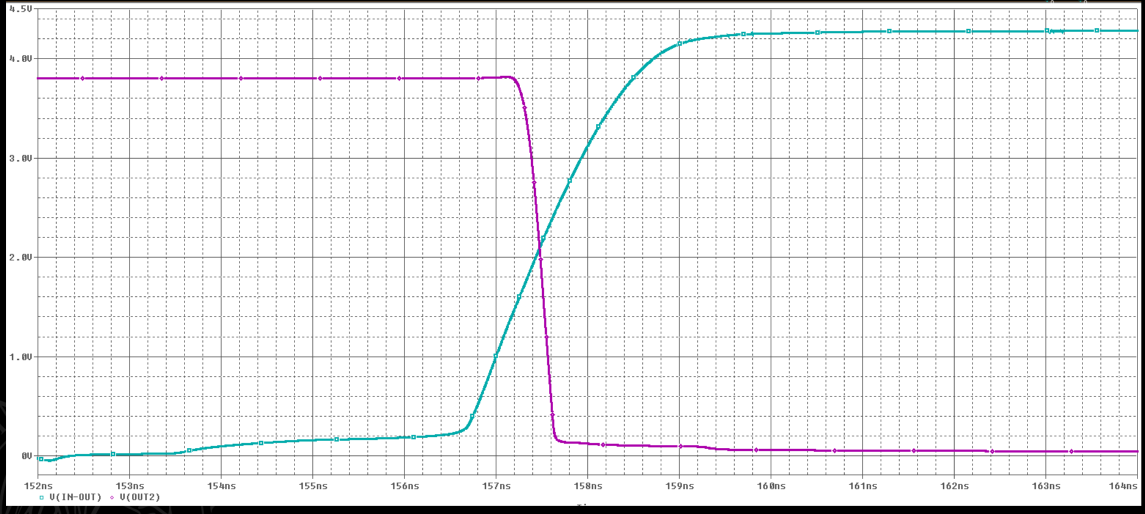
\includegraphics[width=0.6\linewidth,height=\textheight,keepaspectratio]{assets/imgs/grafico_commutazione_h_l.png}
\caption{Grafico commutazione H-L.}
\end{figure}

\begin{itemize}
\item
  \textbf{\emph{Commutazione L-H (Basso \(\to\) Alto)}}

  \begin{itemize}
  \tightlist
  \item
    Da:

    \begin{itemize}
    \tightlist
    \item
      Q2, Q3, Q5 in saturazione;
    \end{itemize}
  \item
    A:

    \begin{itemize}
    \tightlist
    \item
      Q1 in saturazione;
    \item
      Q4 in regione attiva;
    \end{itemize}
  \end{itemize}

  È più difficile rispetto alla commutazione H-L. Quando la tensione in
  ingresso è pari ad un livello logico basso, il transistor Q1 prima di
  passare alla regione di saturazione passa dalla regione attiva diretta
  (a causa delle cariche accumulate sulla base del transistor Q3),
  svuotando così Q3, che si spegnerà.

  \begin{figure}[H]
    \centering
    \resizebox{0.25\textwidth}{!}{\begin{tikzpicture}
	% Paths, nodes and wires:
	\draw node[npn, rotate=-90, xscale=1.25, yscale=1.25] (N1) at (3, 6) {} node[anchor=north] at (N1.text){$Q1$};
	\draw node[circ] at (4, 6) {};
	\draw node[npn, xscale=1.25, yscale=1.25] (N2) at (5.05, 6) {} node[anchor=west] at (N2.text){$Q3$};
	\draw[-stealth] (4, 6) -| (4, 8);
	\node[shape=rectangle, inner sep=0, minimum width=2.965cm, minimum height=0.965cm] at (4, 8.75){} node [anchor=center, align=center, text width=2.577cm, inner sep=5.5pt] at (4, 8.75){$1,4V$,  dalla carica accumulata};
	\node[shape=rectangle, inner sep=0, minimum width=0.965cm, minimum height=0.465cm](Rect1) at (1.5, 6){} node[anchor=center] at (Rect1.center){$Low$};
\end{tikzpicture}}
    \caption{Ingresso basso TTL.}
    \end{figure}

  Ora Q4 si può accendere, mentre il transistor Q2 deve essere
  spento\footnote{Va svuotato dalle cariche!}: questa azione è svolta o
  dalla resistenza di pull-down o dall'\emph{active pull-down} se
  presente. Infatti la presenza o meno del sottocircuito APD gioca un
  ruolo chiave nello spegnimento del transistor.
\end{itemize}

\paragraph{Assenza sottocircuito active
pull-down}\label{assenza-sottocircuito-active-pull-down}

Siamo nel caso in cui vi è solo una resistenza di pull-down. La
commutazione tra lo stato basso e lo stato alto avviene in un tempo
compreso tra i 10 e i 12 nS. \newline Il transistor Q1 svuota la base
del transistor Q3, il quale si spegne. Quando ciò accade la corrente si
sposta verso Q4, il quale si accende e tenta di ``alzare - tirare su''
l'uscita. Tuttavia Q2 deve ancora spegnersi, dal momento che era in
saturazione. Una svolta spento Q2, l'uscita è libera di salire. \newline
Vi è un periodo di tempo in cui sono accesi sia lo stato alto che lo
stato basso; inoltre ho un assorbimento di corrente per tutto
l'intervallo tempo in cui il transistor Q2 non si è ancora spento
(ovvero in quell'arco di tempo in cui il segnale \textbf{non} sta
commutando), comportando un maggior consumo di potenza. Ciò è dovuto
dall'accensione di Q4 e da Q2 non ancora spento, a causa della
cross-conduction.

\begin{figure}
\centering
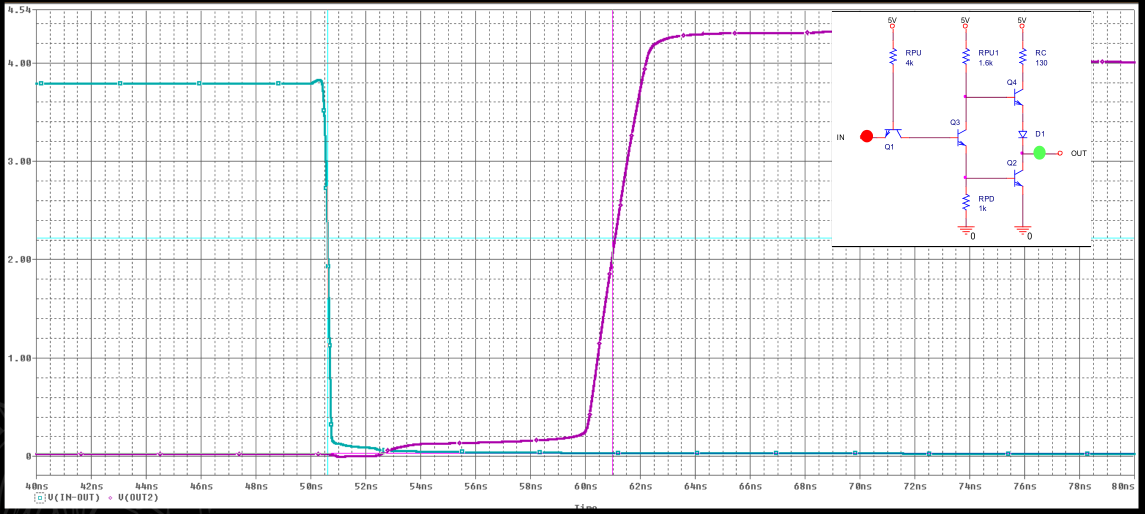
\includegraphics[width=0.6\linewidth,height=\textheight,keepaspectratio]{assets/imgs/commutazione_l_h_no_apd.png}
\caption{Grafico commutazione porta NOT in TTL senza la presenza
dell'APD.}
\end{figure}

\begin{figure}
\centering
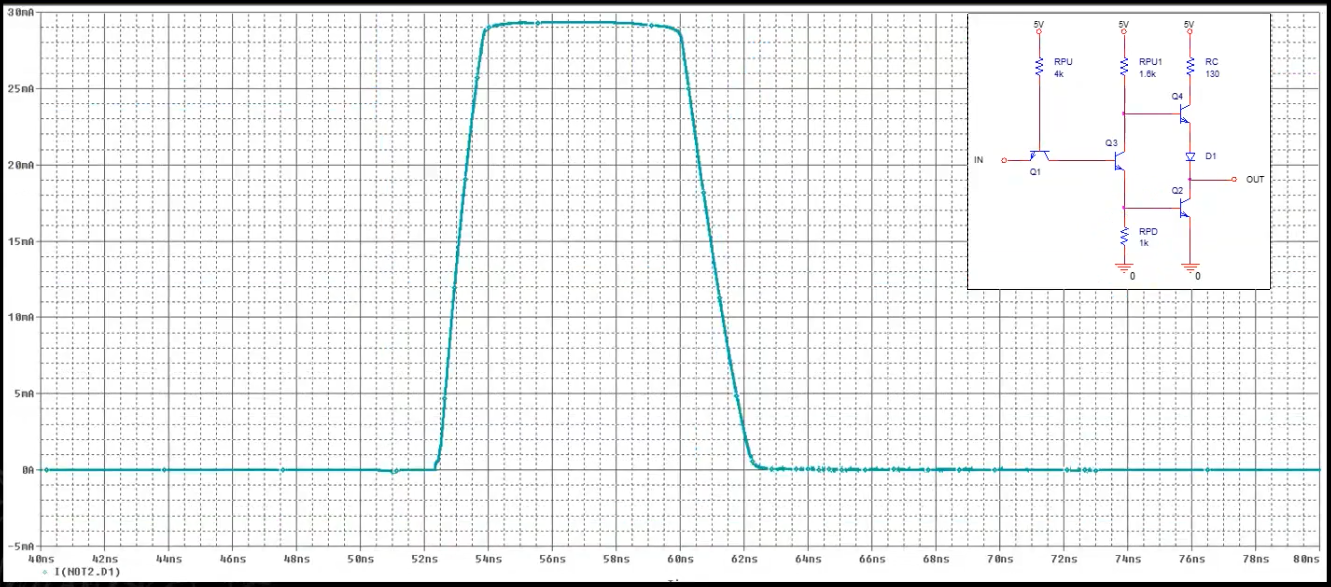
\includegraphics[width=0.6\linewidth,height=\textheight,keepaspectratio]{assets/imgs/corrente_no_apd.png}
\caption{Grafico della corrente porta NOT senza APD.}
\end{figure}

\paragraph{Presenza sotto circuito active
pull-down}\label{presenza-sotto-circuito-active-pull-down}

Il funzionamento dei transistor Q2, Q3, Q5 è sincronizzato sia in
accensione che in spegnimento ed in quest'ultima fase anche
\emph{velocizzato}. Il transistor Q1 svuota sempre la base di Q3, il
quale si spegne. Il tempo necessario al transistor Q2 per spegnersi è
molto inferiore grazie alla presenza di Q5, il quale è un \emph{carico
attivo} e ``tira'' corrente molto velocemente. \newline Il picco di
corrente in questo caso ha una durata più limitata (non più
\(\sim 10nS\)) ed ho quindi un minor consumo di potenza.

\begin{figure}
\centering
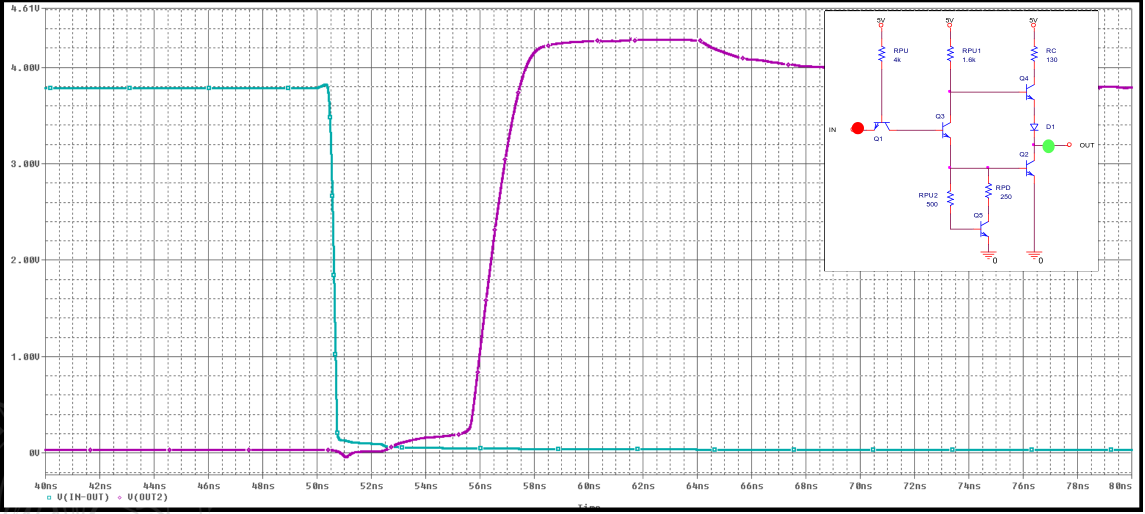
\includegraphics[width=0.6\linewidth,height=\textheight,keepaspectratio]{assets/imgs/commutazione_l_h_apd.png}
\caption{Grafico commutazione L-H porta NOT con APD.}
\end{figure}

\begin{figure}
\centering
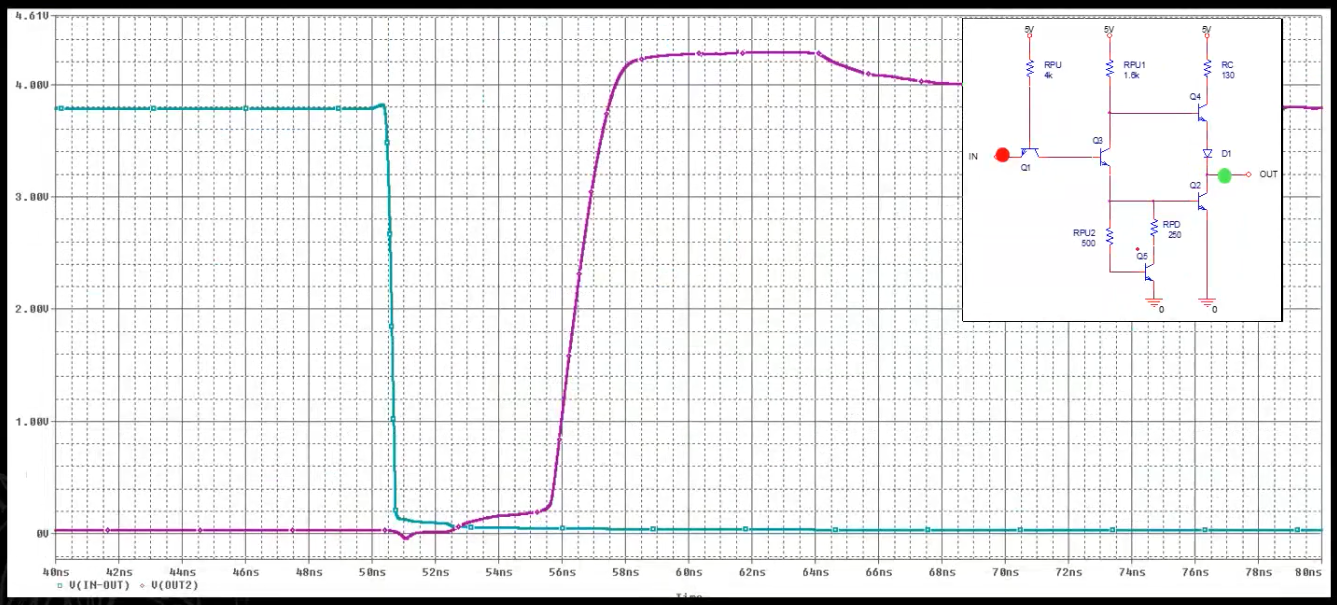
\includegraphics[width=0.6\linewidth,height=\textheight,keepaspectratio]{assets/imgs/corrente_apd.png}
\caption{Grafico assorbimento corrente in presenza di APD.}
\end{figure}

\section{MOS logic cell - Porte logiche
MOS}\label{mos-logic-cell---porte-logiche-mos}

Questa famiglia logica non usa più transitor bipolari, ma passa ai
MOSFET: in questo caso si utilizzando i MOSFET \textbf{\emph{ad
arricchimento}}, come descritti nel paragrafo a loro dedicato. Tuttavia
esistono anche i MOSFET \textbf{\emph{a svuotamento}}, i quali
funzionano in modo inverso, in quanto il canale è già presente e si va
ad applicare una corrente per rimuoverlo.

\subsection{CMOS - Complementary MOS}\label{cmos---complementary-mos}

Andiamo ora a descrivere una famiglia detta \textbf{\emph{Complementary
MOS}} o CMOS, questo perché vengono utilizzati entrambe le tipologie di
transistor ad effetto di campo, sia quelle a canale n sia quelle a
canale P. Un vantaggio nell'utilizzo di transistor MOS per realizzare
porte logiche è la possibilità di realizzare dispositivi molto compatti
e che consumano meno rispetto alle precedenti famiglie logiche.

Le equazioni che guidano la corrente sono:

\subsubsection{CMOS - NOT}\label{cmos---not}

\begin{figure}[H]
    \centering
    \resizebox{0.5\textwidth}{!}{\begin{circuitikz}[american]
	\ctikzset{tripoles/mos style/arrows}
	% Paths, nodes and wires:
	\draw node[nmos] (N1) at (3, 6.25) {} node[anchor=west] at (N1.text){$QN$};
	\draw node[pmos] (N2) at (3, 7.75) {} node[anchor=west] at (N2.text){$QP$};
	\draw (2, 7.75) |- (1.5, 7.75) -| (1.5, 6.25) -- (2, 6.25);
	\draw node[circ] at (1.5, 7) {};
	\draw (1.5, 7) -- (0.5, 7);
	\draw node[ocirc] (N3) at (0.5, 7) {} node[anchor=east] at (N3.west){$v_{in}$};
	\draw node[ground] at (3, 5.48) {};
	\draw[-stealth] (3, 8.5) -| (3, 9);
	\node[shape=rectangle, inner sep=0, minimum width=0.465cm, minimum height=0.465cm](Rect1) at (7, 11){} node[anchor=center] at (Rect1.center){$V_{DD}$};
	\draw node[circ] at (3, 7) {};
	\draw (2, 7.75) -- (2.02, 7.75);
	\draw (2, 6.25) -- (2.02, 6.25);
	\draw (3, 7) -- (4.5, 7);
	\draw node[ocirc] (N4) at (4.5, 7) {} node[anchor=west] at (N4.east){$v_{o}$};
	\node[shape=rectangle, inner sep=0, minimum width=1.465cm, minimum height=0.465cm](Rect2) at (1.25, 8.25){} node[anchor=center] at (Rect2.center){$\text{P-MOS}$};
	\node[shape=rectangle, inner sep=0, minimum width=1.465cm, minimum height=0.465cm](Rect3) at (1.25, 5.75){} node[anchor=center] at (Rect3.center){$\text{N-MOS}$};
	\draw (7, 10.51) to[american resistor, l={$R_{DSP}$}, label distance=0.02cm] (7, 8.51);
	\draw (7, 8.51) to[opening switch, l={$S_{P}$}, label distance=0.02cm, mirror] (7, 7.51);
	\draw (7, 5.505) to[american resistor, l={$R_{DSN}$}, label distance=0.02cm] (7, 3.505);
	\draw (7, 5.505) to[switch, l_={$S_{N}$}, label distance=0.02cm] (7, 6.505);
	\draw node[ground] at (7, 3.505) {};
	\draw (7, 7.51) -- (7, 6.505);
	\draw node[circ] at (7, 7) {};
	\draw (7, 7) -- (8, 7);
	\draw node[ocirc] (N5) at (8, 7) {} node[anchor=west] at (N5.east){$v_{o}$};
	\draw[-stealth] (7, 10.5) -| (7, 10.75);
	\node[shape=rectangle, inner sep=0, minimum width=0.465cm, minimum height=0.465cm](Rect4) at (3, 9.25){} node[anchor=center] at (Rect4.center){$V_{DD}$};
	\draw[-stealth] (3.25, 7.25) -- (3.75, 7.25);
	\node[shape=rectangle, inner sep=0, minimum width=0.465cm, minimum height=0.465cm](Rect5) at (4, 7.25){} node[anchor=center] at (Rect5.center){$I_{D}$};
\end{circuitikz}
}
    \caption{Porta NOT in logica CMOS.}
\end{figure}

Possiamo quindi apprezzare la \emph{simmetria del circuito}, che
contribuisce a semplificarne la gestione.

In base al valore del segnale in ingresso \(v_{i}\) il circuito equivale
alla configurazione sulla destra della figura con:

\appendix

\chapter{Esercizi}\label{esercizi}

\section{Esercizi capitolo 1}\label{esercizi-capitolo-1}

\begin{figure}[h]
\centering
\begin{circuitikz}[american]
\draw[V={}](2.0,-2.5)to(2.0,-5.5);
\draw[D={}](2.0,-2.5)to(6.5,-2.5);
\draw[R={}](6.5,-2.5)to(6.5,-5.5);
\draw[short={}](2.0,-5.5)to(6.5,-5.5);
\end{circuitikz}
\end{figure}

\chapter{Varie}\label{varie}

\begin{bluebox}{Le leggi di Kirchoff}
\begin{enumerate}
\item \emph{Legge di Kirchoff alle correnti}: la somma delle correnti in un nodo è pari a 0.
\item \emph{Legge di Kirchoff alle tensioni}: la somma delle tensioni lungo un percorso chiuso è pari a0.
\end{enumerate}
\end{bluebox}

\section{Semiconduttori e bande}\label{semiconduttori-e-bande}

Gli elettroni in un solido allo stato fondamentale e a temperatura \(0\)
kelvin, in obbedienza alla loro natura fermionica e al principio di
Pauli che preclude ai fermioni il fatto di potersi trovare in due nello
stesso stato, riempiono gli stati elettronici loro consentiti partendo
dal livello energetico più basso via via su, fino a che tutti gli
elettroni del solido hanno trovato un'accomodazione. Si distribuiscono
cioè rispettando la distribuzione di Fermi-Dirac calcolata a temperatura
0 kelvin. Nei metalli, il livello energetico più alto occupato si
definisce livello di Fermi.

\begin{figure}
\centering
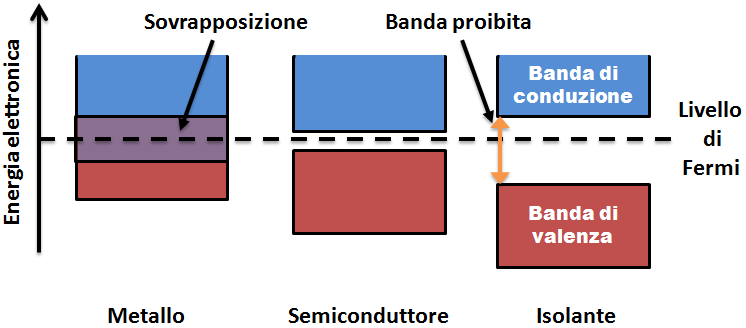
\includegraphics[width=0.5\linewidth,height=\textheight,keepaspectratio]{immagini/bande.png}
\caption{Schema semplificato della struttura elettronica a bande per
metalli, semiconduttori e isolanti.}
\end{figure}

A questo punto possono verificarsi diverse possibilità:

\begin{itemize}
\tightlist
\item
  Vi è una banda, o più di una fra le ultime riempite da elettroni, che
  è parzialmente riempita e restano degli stati vuoti. In tal caso si ha
  a che fare con un metallo, cioè un sistema in cui gli ultimi elettroni
  hanno la possibilità di spostarsi in livelli energetici molto vicini,
  infinitesimalmente più alti in energia, e dunque hanno la possibilità
  di una mobilità elevata che porta il sistema ad essere un buon
  conduttore di elettricità.
\item
  L'ultima banda è stata riempita completamente in modo tale che il
  prossimo stato elettronico consentito si trovi sulla banda successiva
  e fra questa banda e la banda completamente riempita c'è una banda
  proibita (\emph{band gap}) di energie. In tal caso il solido è un
  dielettrico.
\item
  Si parla infine di semiconduttore nel caso di un isolante in cui la
  banda proibita è talmente piccola che a temperatura ambiente c'è una
  certa probabilità che gli elettroni si trovino a saltare la banda
  proibita per agitazione termica, e dunque il sistema si trovi in una
  situazione prossima a quella di un metallo, con valori di
  conducibilità elettrica non nulli.
\end{itemize}

(N.B paragrafo proveniente da
\href{https://it.wikipedia.org/wiki/Struttura_elettronica_a_bande}{Wikipedia})

\begin{comment} 
TODO capire come funziona tavola periodica
## Tavola periodica

%%\pgfPT[show title=false, back color scheme=example,
%%  legend box={draw=blue!50,fill=blue!20},
%%  show extra legend,
%%  Z list={5,7,13,14,15,31,32,33,49,51}]
\end{comment}

\section{Corrente nel N-MOS}\label{corrente-nel-n-mos}

A differenza del transistor BJT, dove la base è comunque ristretta,
abbiamo in pratica due giunzioni p-n tra la base e il source oppure con
il drain: quindi è come se ci fossero due diodi contrapposti. Infatti
ciò spiega il perché in prima approssimazione non scorre corrente tra
Source e Drain (in condizione di quiete).

\section{Termini}\label{termini}

\begin{itemize}
\tightlist
\item
  \(V_{cc}\): è la tensione di alimentazione positiva che fornisce
  energia a un circuito elettronico associata al collettore; sta per
  ``Voltage at the Common Collector'' (tensione al collettore comune),
  che è il punto di riferimento per le tensioni di alimentazione nei
  circuiti a transistor bipolari (BJT).
\item
  Le \textbf{\emph{resistenze di pull-up e pull-down}} sono usate nei
  circuiti logici elettronici per garantire che gli ingressi di un
  sistema logico stabilito siano a livelli logici previsti se i
  dispositivi esterni sono scollegati o ad alta impedenza. Essi possono
  essere utilizzati anche a livello di interfaccia tra due diversi tipi
  di dispositivi logici, possibilmente operanti a diverse tensioni di
  alimentazione.

  \begin{table}[H]
    \centering
    \resizebox{\textwidth}{!}{
        \begin{tabular}{|c|c|c|}
        \hline
        \textbf{Uscita del segnale/interruttore}                      & \textbf{Interruttore aperto}                                   & \textbf{Interruttore chiuso}                                                   \\ 
        \hline
        \textbf{Con resistore di pull-up}                             & Tensione di alimentazione positiva / segnale alto              & Tensione di massa / segnale basso                                              \\ 
        \hline
        \textbf{Con resistore di pull-down}                           & Tensione di massa / segnale basso                              & Tensione di alimentazione positiva / segnale alto                              \\ 
        \hline
        \textbf{Senza resistore di pull-up o pull-down}               & Tensione/segno indeterminato                                   & Tensione/segno dell'ingresso dell'interruttore                                 \\
        \hline
        \end{tabular}
    }
    \caption{Tabella di comportamento del segnale dell'interruttore con vari resistori}
  \end{table}
\end{itemize}

\backmatter
\end{document}
